\section{Geometría y Ciclo Operativo del MRCVC}
%
En esta sección se describen algunos de los aspectos geométricos del motor y
ciclo operativo del MRCVC.

Los componentes principales del motor son: rotor, estator, paletas, bieletas,
rueda paralelizadora, eje motor, conducto de admisión y conducto de escape.
%
El motor analizado en este trabajo tiene 3 paletas con ápices agudos, que
corresponden a la geometría ideal del motor (ápices de paletas de radio nulo).
%
Estos elementos se esquematizan en la Figura~\ref{fig:geom_flor_mrcvc}.
%
En la Tabla~\ref{tab:geom_mrcvc} se resume el valor de los parámetros
geométricos utilizados en este trabajo.

Uno de los aspectos más importantes de este motor es la geometría de la cámara
de combustión.
%
Su forma es tal que el volumen mínimo del ciclo permanece constante por un
período angular considerable. % , determinado por la geometría del motor.
%
Este período es lo suficientemente grande para permitir que la combustión
ocurra casi en su totalidad a volumen constante, como se observa en las
Figuras~\ref{fig:mrcvc_vol_cte} y~\ref{fig:PV_mrcvc}.
%
Este tipo de combustión brinda una mejora en el rendimiento energético del
motor, además el balanceo de fuerzas que se obtiene por ser un motor rotativo
permite operar el motor a altas RPM y así alcanzar mayores potencias en
comparación a motores alternativos de tamaño o cilindrada similar.
%
Esta combinación de rendimiento y potencia que, en principio pueden ser
relativamente altos, hace atractivo el desarrollo de este motor.
%

\begin{figure}[ht]
  \centering
  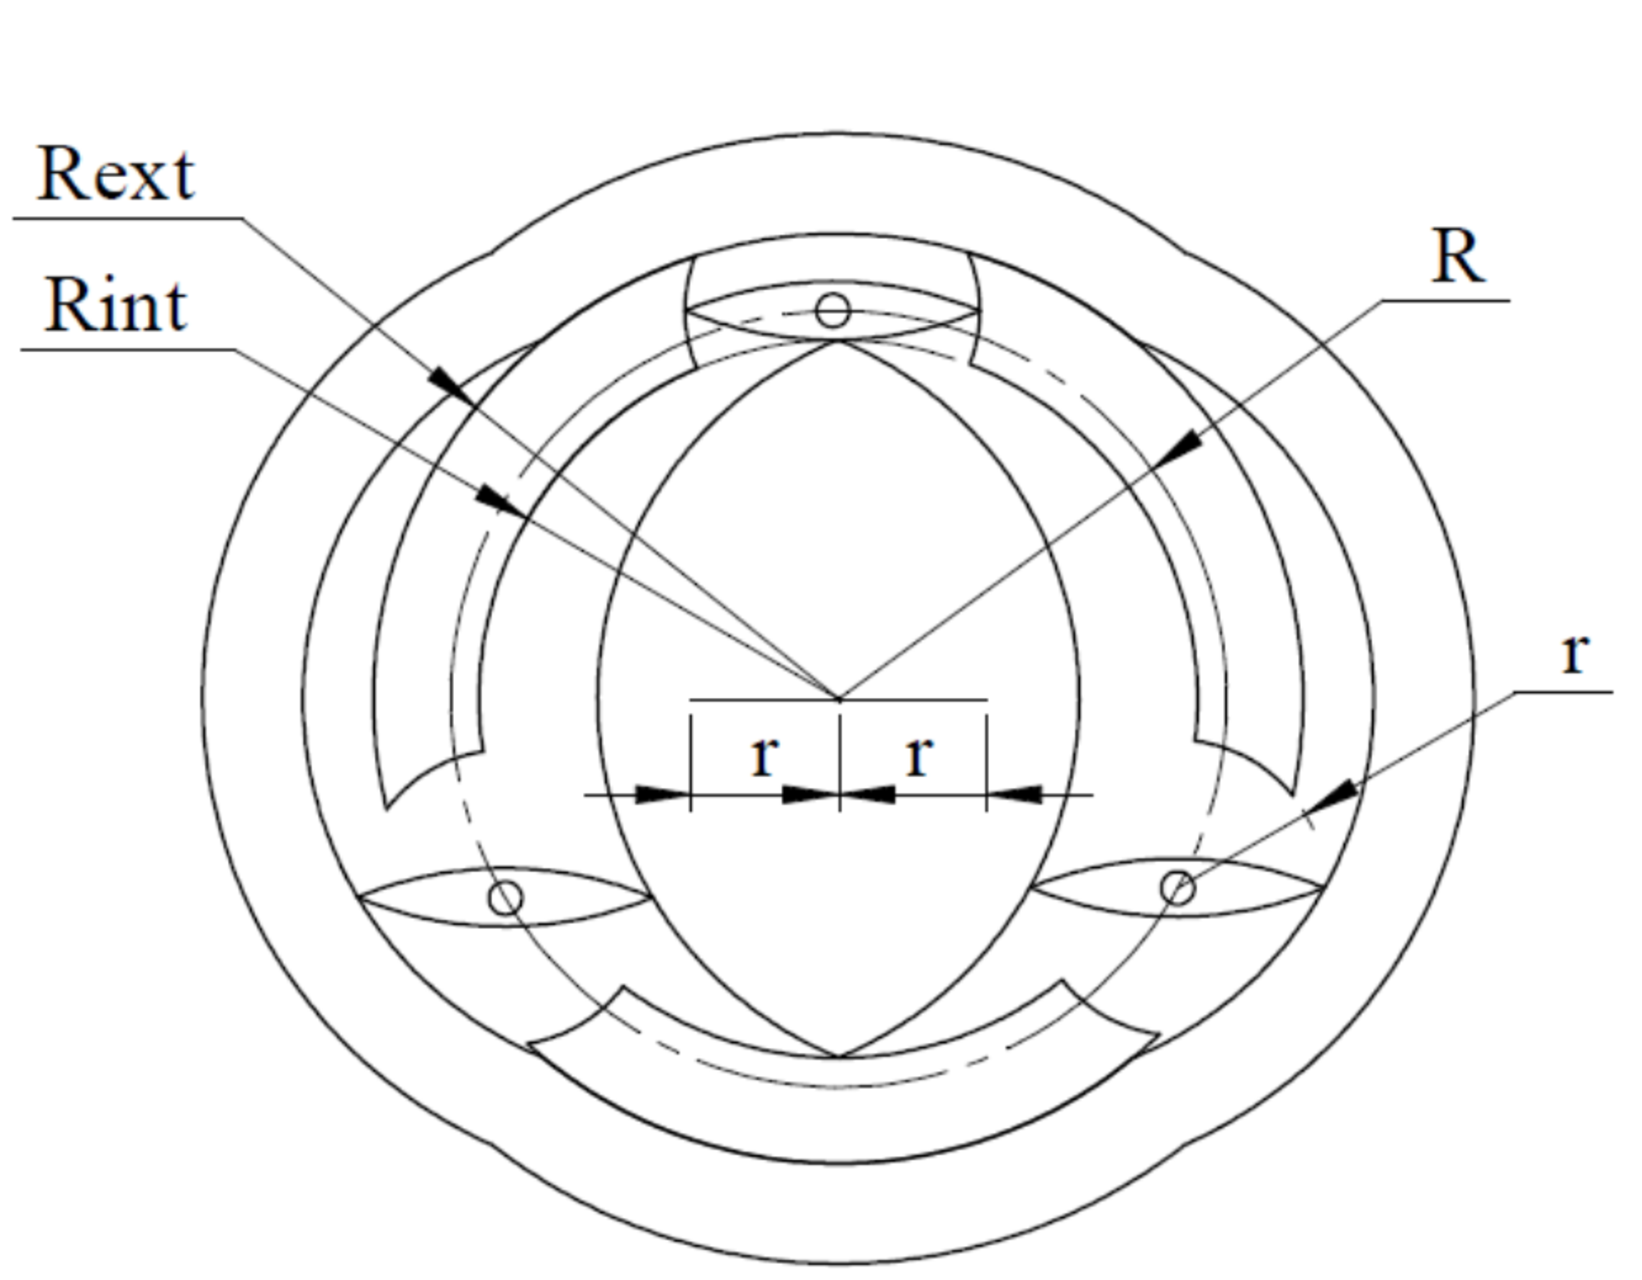
\includegraphics[width=0.7\textwidth]{plano_mrcvc_flor.pdf}
  \caption{Parámetros goemétricos del MRCVC~\parencite{roldan}}\label{fig:geom_flor_mrcvc}
\end{figure}

\begin{figure}[ht]
  \centering
  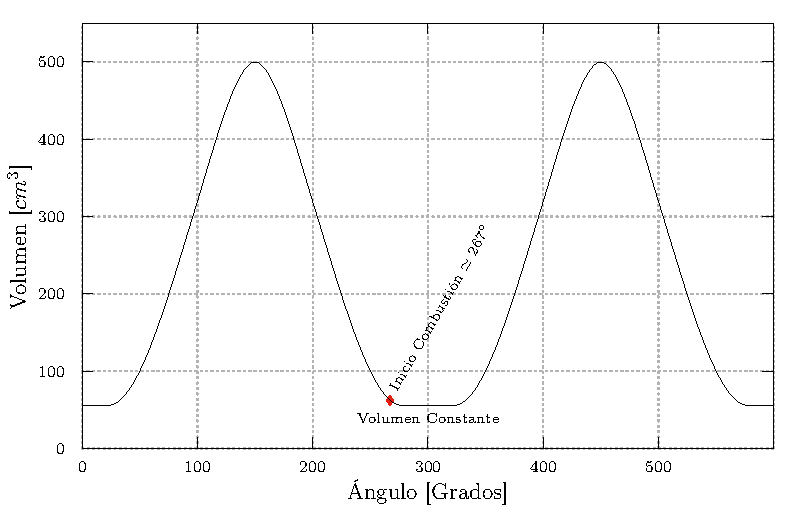
\includegraphics[width=0.7\textwidth]{gnuplot/vol.pdf}
  \caption{Variación del volumen del MRCVC}\label{fig:mrcvc_vol_cte}
\end{figure}

\begin{figure}[ht]
  \centering
  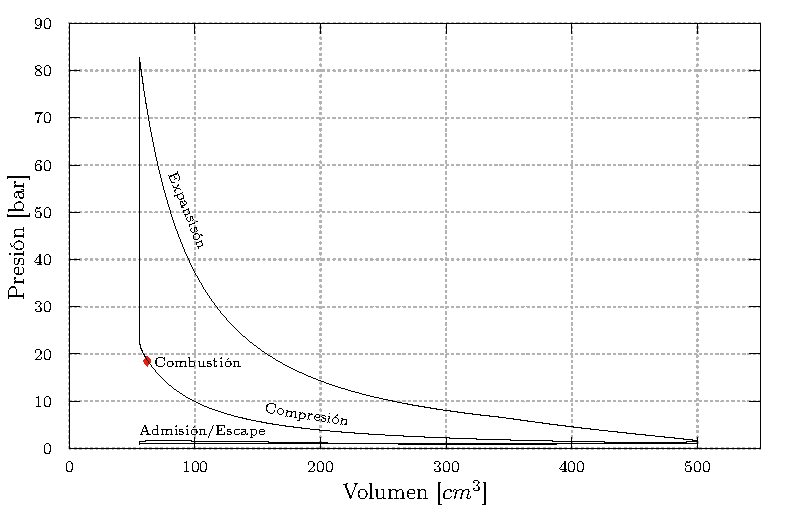
\includegraphics[width=0.7\textwidth]{gnuplot/vol_vs_pres.pdf}
  \caption{Ciclo operativo del MRCVC}\label{fig:PV_mrcvc}
\end{figure}

El ciclo operativo ideal del MRCVC es considerado un ciclo Otto en el que las
carreras de admisión, compresión, expansión y escape ocurren a medida que el
fluido de trabajo rota con respecto al eje del cigüeñal.
%
En la Figura~\ref{fig:ciclo_mrcvc} se puede ver una progresiva del ciclo del
MRCVC con estas carreras representadas en azul para la admisión, compresión en
amarillo, expansión en rojo y escape o barrido en violeta.

Durante el ciclo se destaca un aspecto particular de este motor, siguiendo la
paleta de color negro se ve que durante el proceso de compresión y combustión,
las paletas que forman la frontera aguas arriba y aguas abajo de la cámara de
combustión cambian.
%
La paleta que delimita el frente de la cámara se adelanta con respecto a la
cámara con la que inició el ciclo, produciendo que este dure más de una
revolución resultando en $600^{\circ}$ de giro del cigüeñal para el caso de 3
paletas considerado en este trabajo.

Para un motor con las características geométricas indicadas en la
Tabla~\ref{tab:geom_mrcvc}, el volumen mínimo alcanzado permanece constante por
un período de $\sim 44,65^\circ$, como se puede ver en la
Figura~\ref{fig:mrcvc_vol_cte} en donde se representa la variación del volumen
con respecto al ángulo de eje.
%
En este gráfico se indica el ángulo de inicio de la combustión, el cual
\emph{es una estimación} basada en datos de otros motores como
$\theta_{0}\simeq 267^{\circ}$.
%
En la Tabla se listan el número de paletas $n$, los radios $R$, $R_{e}$,
$R_{i}$ y $r$, altura de cámara $h_{c}$, altura de puerto $h_{p}$, relación de
compresión $r_{c}$


\begin{figure}[ht]
  \centering
  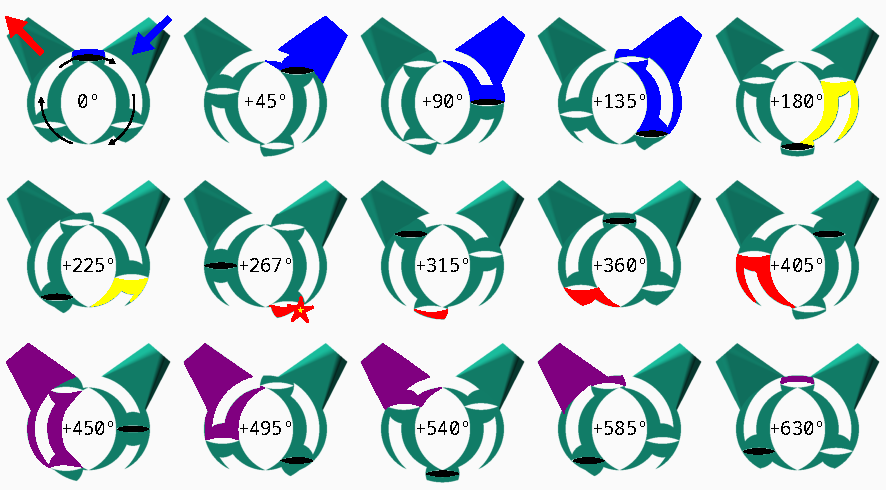
\includegraphics[width=\textwidth]{ciclo/ciclo_operativo.pdf}
  \caption{Ciclo operativo del MRCVC}\label{fig:ciclo_mrcvc}
\end{figure}

\begin{table}
    \centering
    \begin{tabular}{rccccccccc} \toprule
        Parámetro & n & R & r & $h_{c}$ & $h_{p}$ & rc & $V_{max}$ & $R_i$ & $R_e$ \\ \midrule
     Valor & \lua{tex.print(myData.n)} & \lua{tex.print(myData.R)} & \lua{tex.print(myData.r)} & \lua{tex.print(myData.hc)} & \lua{tex.print(myData.hp)} & \lua{tex.print(myData.rc)} & \lua{tex.print(myData.V0)} & \lua{tex.print(trunc(myData.Ri))} & \lua{tex.print(trunc(myData.Re))} \\
     Unidades & --- & mm & mm & mm & mm & --- & $cm^3$ & mm & mm \\ \bottomrule
    \end{tabular}
    \caption{Datos de la geometría del MRCVC considerados en el trabajo}\label{tab:geom_mrcvc}
\end{table}

\nomenclature[G]{\(R\)}{Radio de referencia del MRCVC, ver Figura \ref{fig:mrcvc_vol_cte}}
\nomenclature[G]{\(R_{i}\)}{Radio de cara interna del rotor del MRCVC, ver Figura \ref{fig:mrcvc_vol_cte}}
\nomenclature[G]{\(R_{e}\)}{Radio de cara externa del rotor del MRCVC, ver Figura \ref{fig:mrcvc_vol_cte}}
\nomenclature[G]{\(r\)}{Radio de trayectoria de paletas, ver Figura \ref{fig:mrcvc_vol_cte}}
\nomenclature[G]{\(n\)}{Número de paletas del MRCVC}
\nomenclature[G]{\(h_c\)}{Altura de cámara}
\nomenclature[G]{\(h_p\)}{Altura de puerto}


%%%%%%%%%%%%%%%%%%%%%%%%%%%%%%%%%%%%%%%%%%%%%%%%%%%%%%%%%%%%%%%%%%%%%%%%%%%%%%%

\subsection{Sistemas de Intercambio de Gases}
%
En un motor típico de combustión interna de encendido por chispa, el sistema de
intercambio de gases se compone de una toma de aire, filtro, cuerpo de
mariposa, conducto y puerto de admisión, conducto y puerto de escape,
catalizador y silenciador hasta finalmente descargar en la atmósfera.

Para simplificar el sistema analizado no se tuvieron en cuenta elementos como:
mariposa, carburador, filtros de aire, convertidores catalíticos y demás; se
utilizó un sistema simplificado en el que solamente se tiene conducto de
admisión y escape junto con puertos de admisión y escape.
%
El eje de los conductos coincide con el eje del puerto, estos últimos hacen una
transición desde el diámetro del conducto hasta la altura de la ranura del
puerto en la cámara de combustión.
%
En la Figura~\ref{fig:sistema_intercambio_gases} se esquematiza la geometría
mencionada.

\begin{figure}
    \centering
    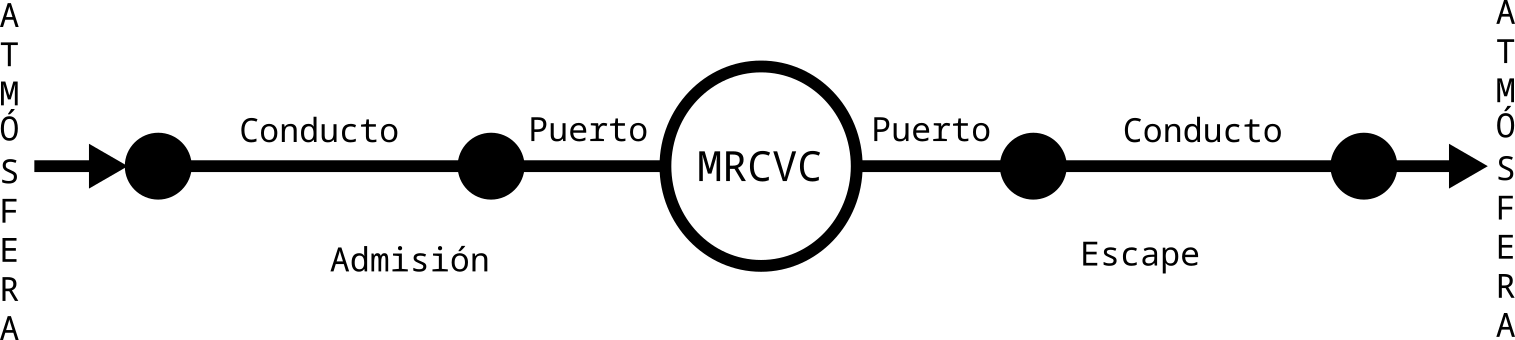
\includegraphics[width=\textwidth]{ciclo/sistema_intercambio_gases.png}
    \caption{Esquema del sistema de intercambio de gases}\label{fig:sistema_intercambio_gases}
\end{figure}


En trabajos anteriores~\parencite{lopez13} se demostró que se tiene una mejor
\emph{performance} del motor si se ubican los puertos en el cuerpo central del
estator, comparado al rendimiento obtenido con los puertos ubicados en las
tapas del mismo.
%
En dicho trabajo se realizó una optimización de la geometría mediante un
barrido paramétrico de las variables que determinan la forma, posición y
reglaje de los puertos, ya que es la ubicación angular de los puertos la que
determina la duración de los procesos de admisión y escape.
%
Los puertos están fijos en la periferia del estator y su posición se define con
los ángulos \emph{IIA}, \emph{IFA} para la admisión y \emph{EIA}, \emph{EFA}
para el escape, ver Figura~\ref{fig:angulos_puertos}.

\nomenclature[G]{\(IIA\)}{Ángulo de apertura del puerto de admisión, ver Figura \ref{fig:angulos_puertos}}
\nomenclature[G]{\(IFA\)}{Ángulo de cierre del puerto de admisión, ver Figura \ref{fig:angulos_puertos}}
\nomenclature[G]{\(EIA\)}{Ángulo de apertura del puerto de escape, ver Figura \ref{fig:angulos_puertos}}
\nomenclature[G]{\(EFA\)}{Ángulo de cierre del puerto de escape, ver Figura \ref{fig:angulos_puertos}}

\begin{figure}
    \centering
    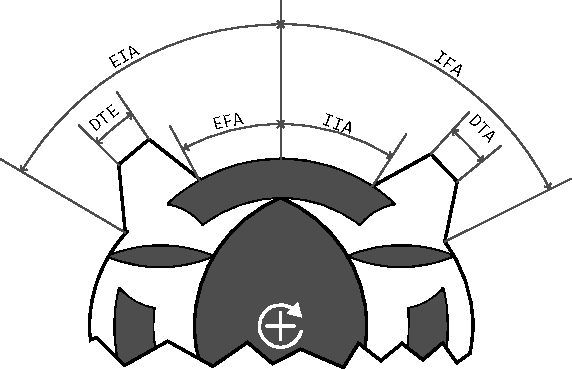
\includegraphics[width=0.6\textwidth]{/CAD/angulos.pdf}
    \caption{Puerto de admisión y escape}\label{fig:angulos_puertos}
\end{figure}

\begin{figure}
\centering
  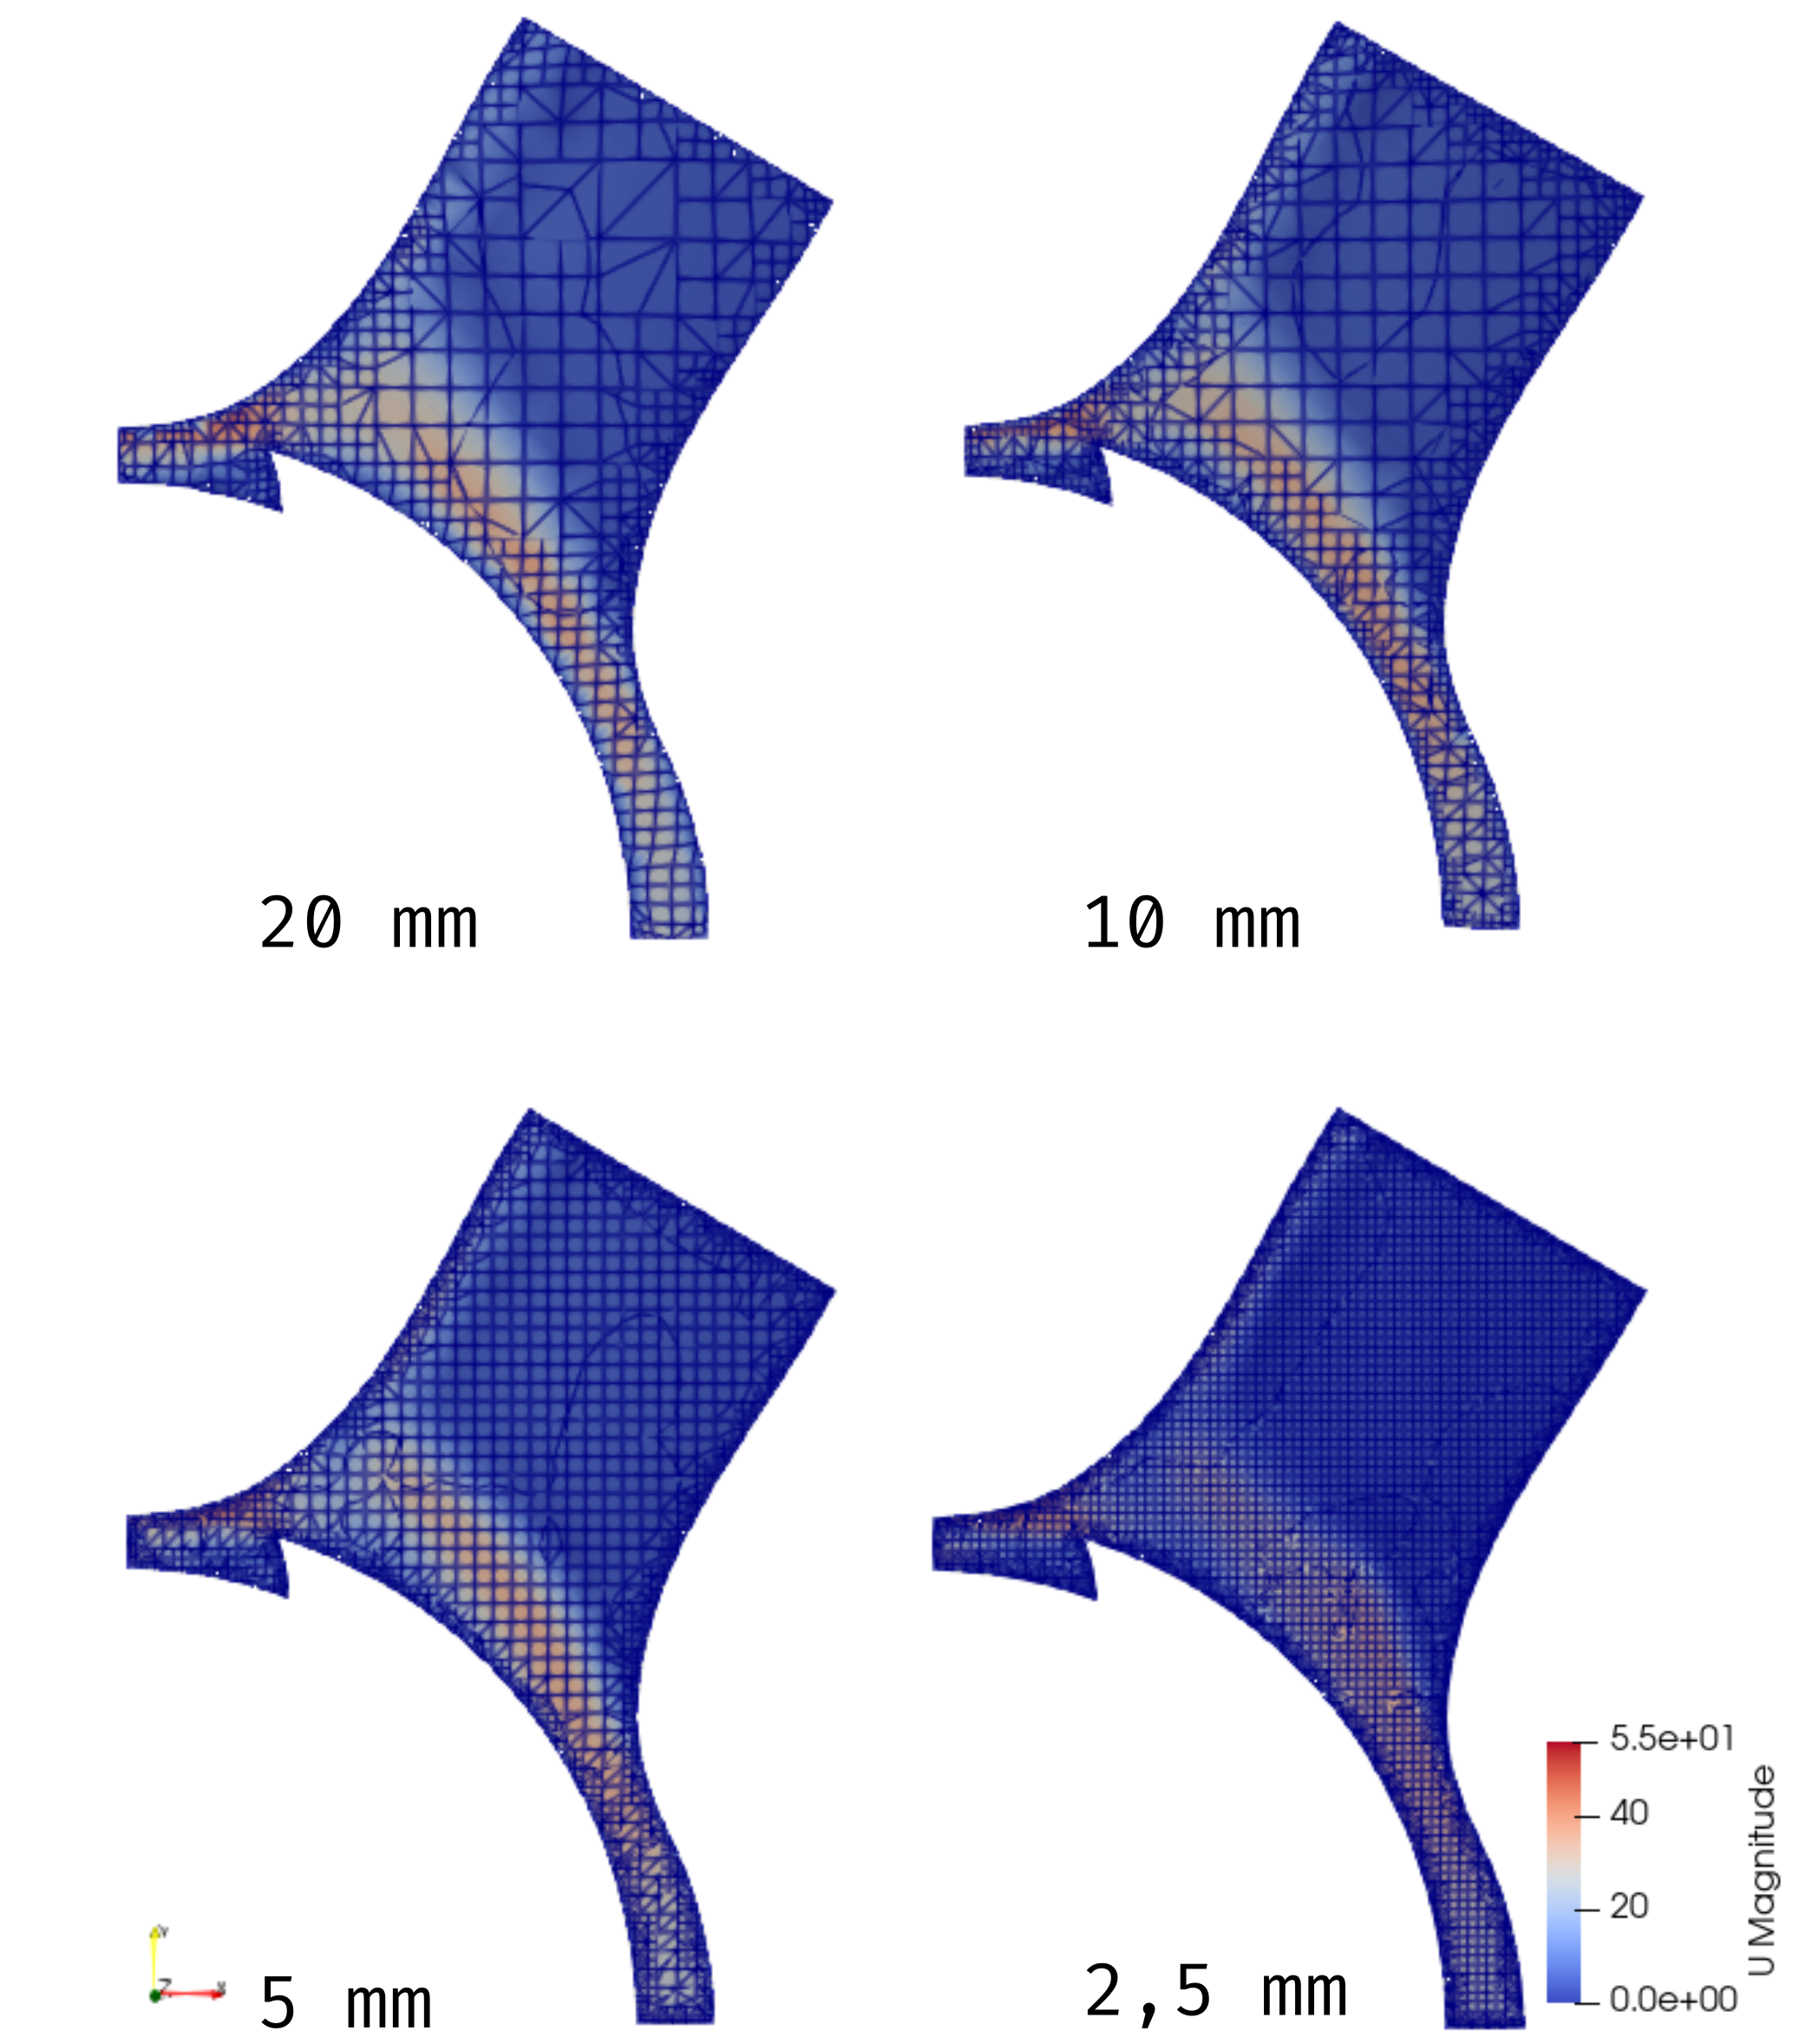
\includegraphics[]{./flujometrias/refinamiento_malla_admision.png}
  \caption{Refinamiento de malla para puerto de admisión}\label{fig:refinamiento_admision}
\end{figure}

\begin{figure}
  \centering
  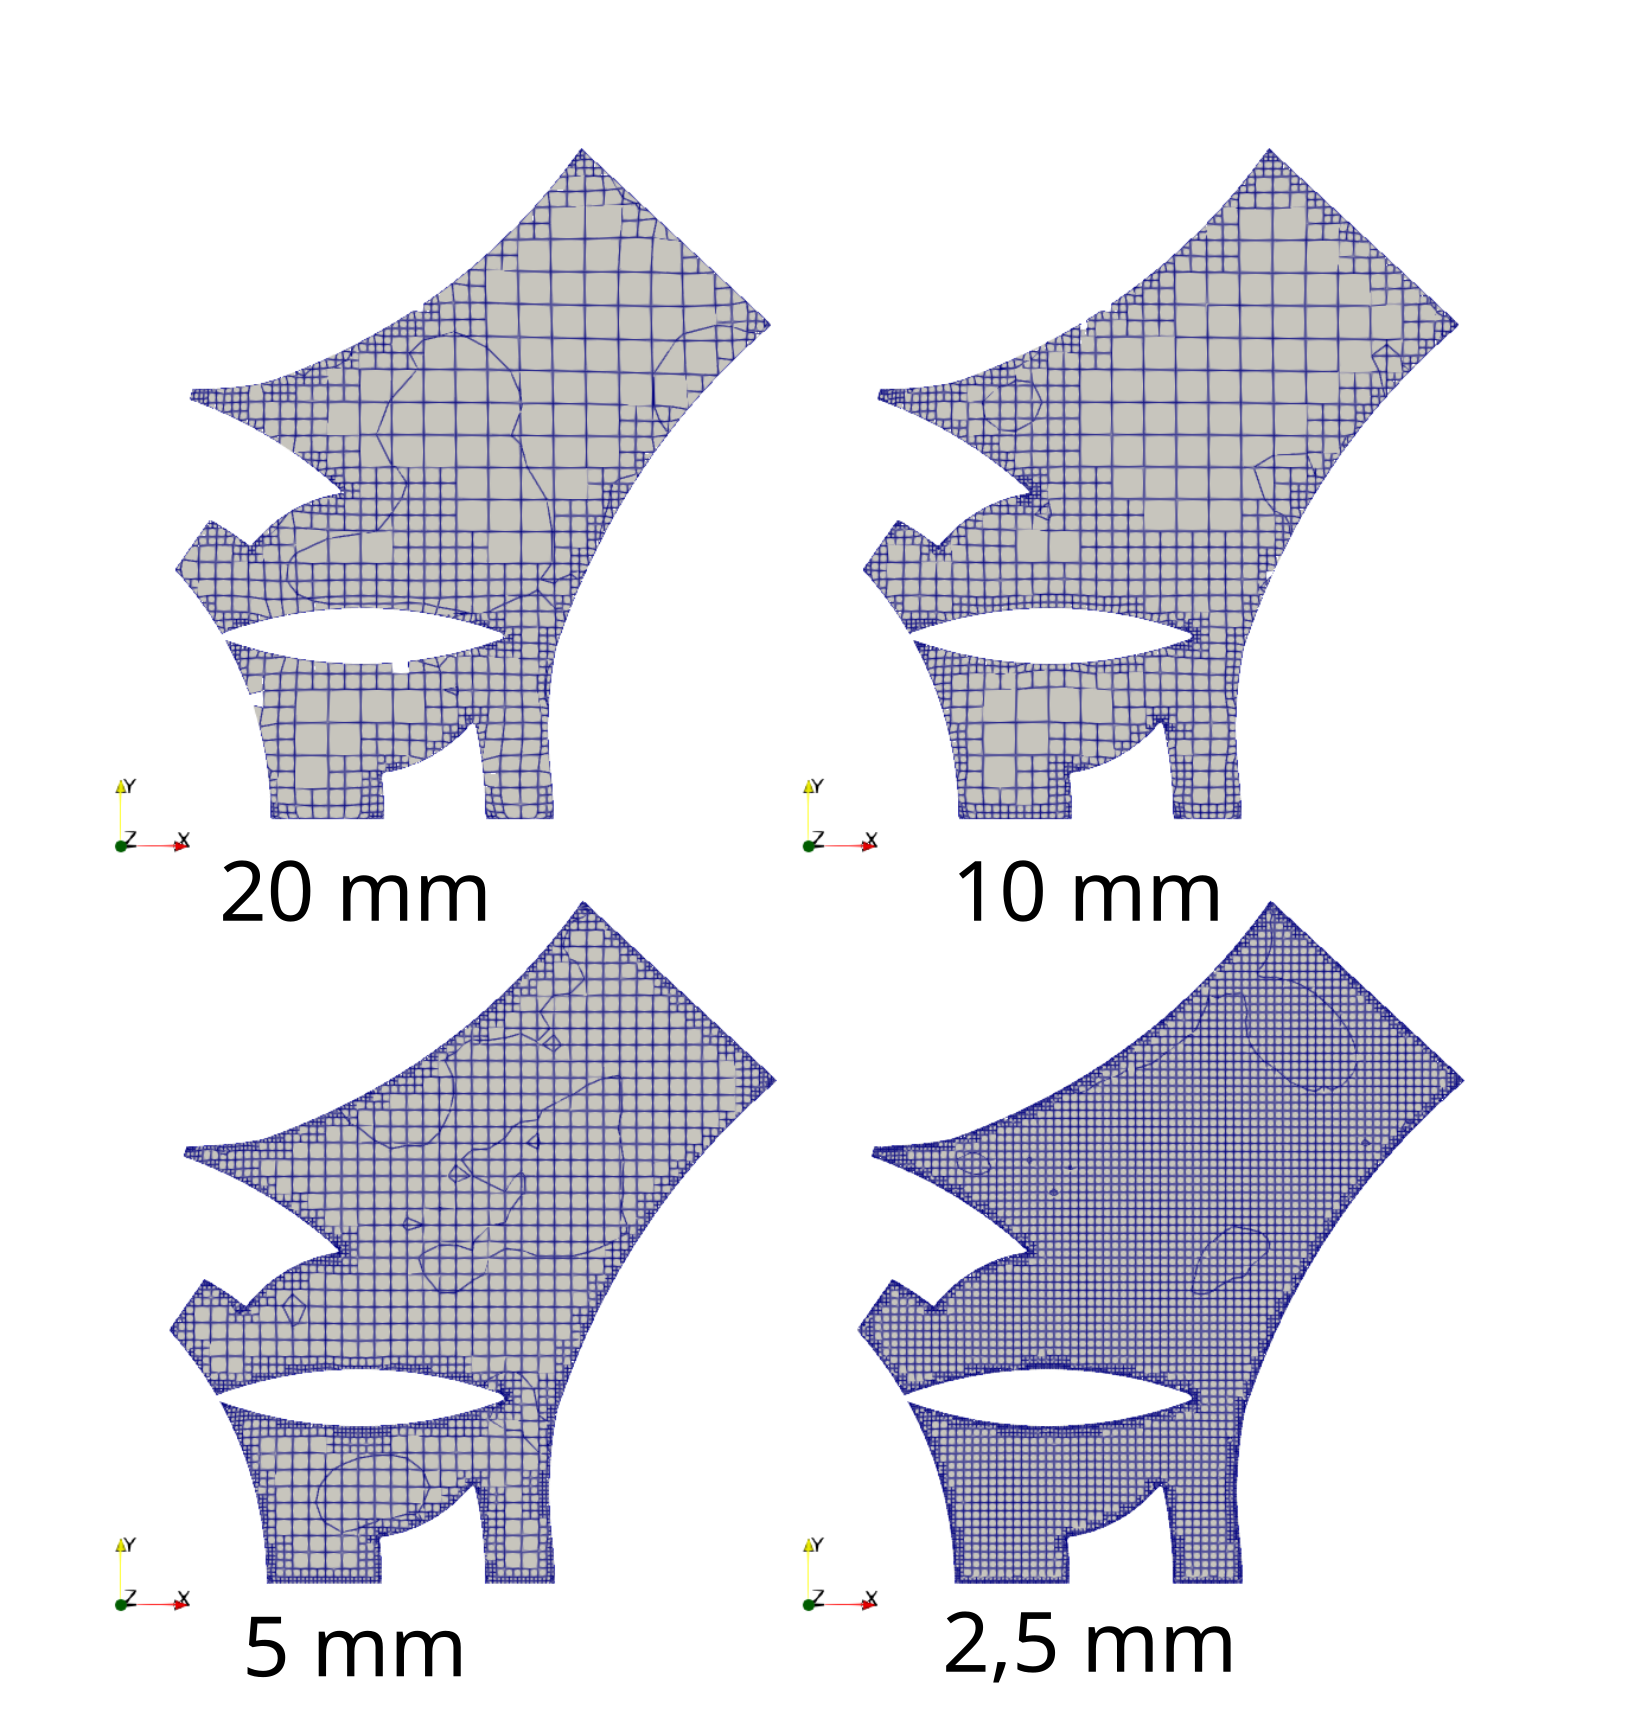
\includegraphics[]{./flujometrias/refinamiento_malla_escape.png}
  \caption{Refinamiento de malla para puerto de escape}\label{fig:refinamiento_escape}
\end{figure}

\begin{figure}
  \centering
  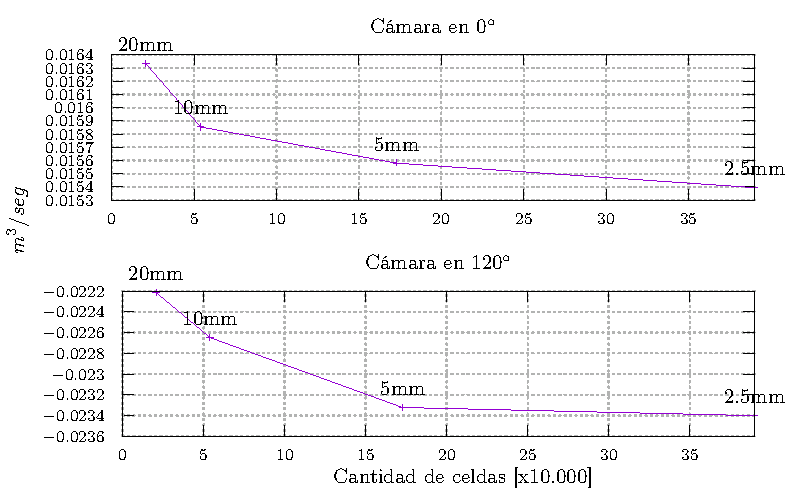
\includegraphics[width=0.9\textwidth]{./flujometrias/convergencia_admision_2000rpm.pdf}
  \caption{Convergencia de malla de puerto de admisión}\label{fig:conv_malla_admision}
\end{figure}

\begin{figure}
  \centering
  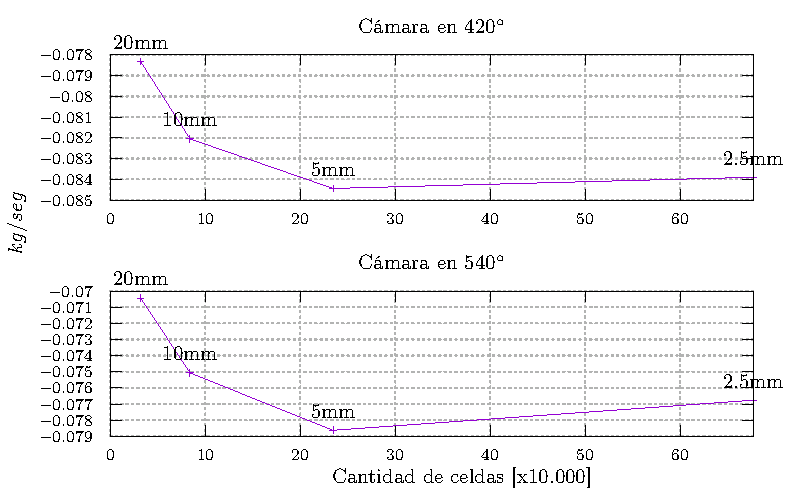
\includegraphics[width=0.9\textwidth]{./flujometrias/convergencia_escape_4000rpm.pdf}
  \caption{Convergencia de malla de puerto de escape}\label{fig:conv_malla_escape}
\end{figure}


Para este trabajo se realizaron las siguientes consideraciones:

\begin{enumerate}
        %
    \item El combustible utilizado es isooctano, la mezcla aire-combustible es
estequiométrica ($\phi=1$).
        %
    \item El sistema de intercambio de gases del MRCVC se compone de un conducto
y puerto admisión, conducto y puerto de escape.
        %
        ICESym tiene en cuenta pérdidas por fricción viscosa en los conductos,
los puertos generan pérdidas localizadas.
        %
    \item Los conductos se asumen como elementos rectos de un largo finito y
diámetro constante, cuya fuente y sumidero es la atmósfera a $101330 Pa$ y
$25^{\circ}C$.
        %
    \item La temperatura de la pared de la cámara de combustión se asume en
450K.
        %
    \item El motor es naturalmente aspirado.
        %
\end{enumerate}
%
\nomenclature[PO]{\(\phi\)}{Relación de equivalencia combustible/aire}

($C_{8}H_{18}$) cuya reacción (estequiométrica) se indica en la
ecuación~(\ref{eq:estequeometrica}).

\begin{equation} \label{eq:estequeometrica}
  C_{8}H_{18} + 12,5 \left(O_{2}+3,772N_{2}\right) \rightarrow 8 CO_{2} + 9 H_{2}O + 47,16 N_{2}
\end{equation}

Expresando el combustible en función de la cantidad de moles de carbono,
$CH_{y}$ con $y=\frac{b}{a}=18/8=2.25$, se puede expresar la proporción
estequiométrica de aire combustible que se requiere con la
ecuación~(\ref{eq:rel_as}):

\begin{equation} \label{eq:rel_as}
  \left(\frac{A}{F}\right)_{s} = \left(\frac{F}{A}\right)_{s}^{-1} = \frac{34,56(4+2.25)}{12,011 + 1,008\cdot 2.25} \simeq 15.127
\end{equation}

\subsection{Área de Referencia}
%
Para el área de referencia ($A_{R}$) se utilizó el área frontal del puerto
expuesta a la cámara, la cual se obtiene del producto de la altura del puerto
$h_{p}$ y la distancia entre una arista del puerto y el extremo de la paleta
(eq.\ref{eq:ar_mrcvc}).
%
La altura de puerto vale $h_{p}=29,4$ mm.

\begin{equation}\label{eq:ar_mrcvc} 
    A_{R,i} = h_{p} \cdot l_{v,i}
\end{equation}

El área de utilizada se ilustra en la Figura~\ref{fig:area_referencia}.
%
Se observan dos zonas coloreadas que hacen referencia al área de dos cámaras
contiuas durante un período de solape de cámaras.


\begin{figure}
  \centering
  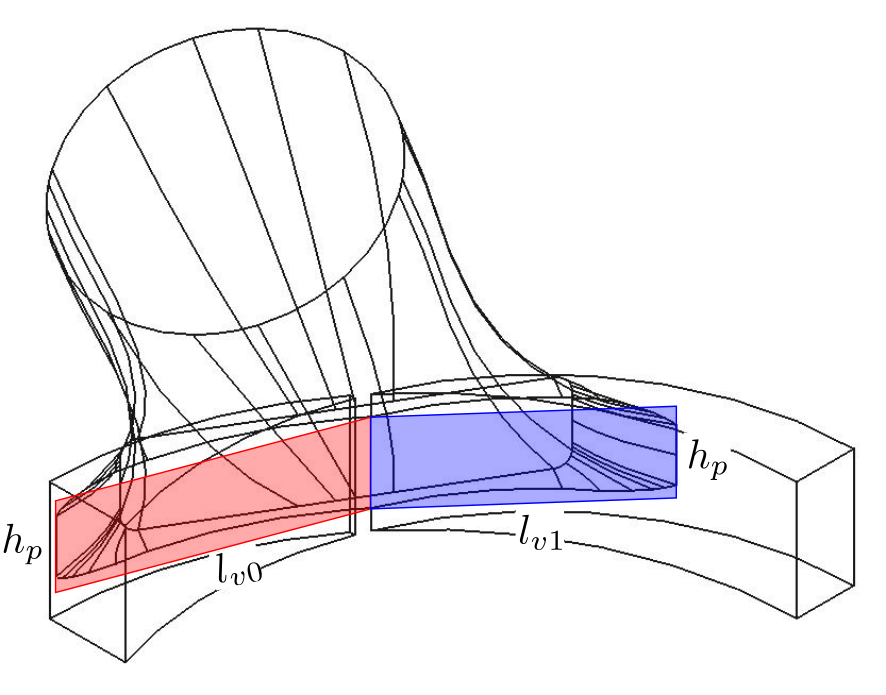
\includegraphics[width=.6\textwidth]{area_referencia.png}
  \caption{Área de referencia MRCVC}\label{fig:area_referencia}
\end{figure}

\subsection{Pérdidas por fricción}

Se incorporaron las pérdidas por rozamiento los sellos de las paletas y sellos
estatóricos del MRCVC utilizando valores obtenidos en trabajos
anteriores~\parencite{roldan}.
%
El trabajo de fricción para diferentes velocidades se consideró en la etapa de
post-procesamiento de las simulaciones de ICESym.

La presión media efectiva de fricción (\textit{fmep}) se obtiene a partir del
trabajo de fricción y el volumen desplazado.

\begin{equation}
  fmep_{cilindro} = \frac{W_{f}}{V_{d}}
\end{equation}

En la Tabla~\ref{tab:trabajo_fricción} se presentan los valores de trabajo de
fricción correspondientes a diferentes regímenes velocidad.

\begin{table}[h!]
  \centering
  \begin{tabular}{cccccccccc}
    \toprule
    \textbf{RPM} & 1000 & 2000 & 3000 & 4000 & 5000 & 6000 & 7000 & 8000 & 9000 \\
    \midrule
    \textbf{$W_{f}$ [J]} & 25.204 & 26.19 & 26.619 & 27.755 & 28.781 & 31.392 & 28.449 & 31.975 & 32.263 \\
    \bottomrule
  \end{tabular}
  \caption{Pérdidas por fricción en sellos de paletas y sellos estatóricos}\label{tab:trabajo_fricción}
\end{table}



\section{Flujometrías Virtuales}
%
Se realizaron una serie de flujometrías para obtener valores de $C_{D}$ en
función de la diferencia de presión a través del puerto y la apertura del
mismo\footnote{ICESym utiliza alzada, por lo que se traduce área de pasaje de
puerto en alzada de válvula equivalente.}, con el fin de obtener un mapa del
coeficiente de descarga en función de la presión y apertura del puerto
($C_{D} = f(\Delta P,l_v)$).
%
ICESym requiere de información del $C_{D}$ para calcular el área efectiva
de pasaje de flujo de las válvulas (o puertos en el caso del MRCVC).
%
Introduciendo el mapa de $C_{D}$ se tiene un mejor modelado del funcionamiento
del sistema de intercambio de gases porque se conoce la pérdida de carga
localizada para un rango de operación del motor.

Para las flujometrías se utilizó el software OpenFOAM seleccionando el algoritmo
PIMPLE, con sus implementaciones ``pimpleFoam'' y ``rhoPimpleFoam'' para los
casos en los que se considera un fluido de trabajo incompresible y compresible
respectivamente.
%
La configuración del software se detalla en la Sección~\ref{sec:3_openfoam}.

\subsection{Modelos de Turbulencia}
%
El flujo a través del puerto es de carácter transitorio, turbulento.
%
Para modelar este tipo de flujo se utilizó el modelo de turbulencia de dos
ecuaciones \emph{$\kappa-\epsilon$}\parencite{wilcox}, que consta de una
ecuación para la \emph{energía cinética turbulenta} $\kappa$ y otra para la
\emph{tasa de disipación de la energía cinética turbulenta} $\epsilon$.
%
El modelo está basado en el modelo estándar
$\kappa-\epsilon$~\parencite{launderSpalding} y es uno de los más populares con
\emph{performance} conocida.
%
Las ecuaciones del modelo son:

\begin{equation}\label{eq:k}
  \frac{D}{Dt}(\rho \kappa) = \nabla \cdot (\rho D_{\kappa}\nabla \kappa) + P_{\kappa} - \rho \epsilon
\end{equation}

\nomenclature[PO]{\(\rho\)}{Densidad}
\nomenclature[F]{\(\kappa\)}{Energía cinética turbulenta}
\nomenclature[F]{\(D_{\kappa}\)}{Difusividad efectiva para $\kappa$}
\nomenclature[F]{\(P_{\kappa}\)}{Tasa de producción de energía cinética turbulenta}
\nomenclature[F]{\(\epsilon\)}{Tasa de disipación de energía cinética turbulenta}

donde

\begin{itemize}
  \item[-] $\kappa$ es la energía cinética turbulenta.
  \item[-] $D_{\kappa}$ es la difusividad efectiva para $\kappa$.
  \item[-] $P_{\kappa}$ es la tasa de producción de energía cinética turbulenta.
  \item[-] $\epsilon$ es la tasa de disipación de energía cinética turbulenta.
\end{itemize}


\begin{equation}\label{eq:k}
  \frac{D}{Dt}(\rho \epsilon) =
  \nabla \cdot (\rho D_{\epsilon}\nabla \epsilon) +
  \frac{C_{1}\epsilon}{\kappa} \left( P_{\kappa}+C_{3}\frac{2}{3}\kappa\nabla\cdot u \right) -
  C_{2}\rho\frac{\epsilon^{2}}{\kappa}
\end{equation}

donde
\begin{itemize}
  \item[-] $D_{\epsilon}$ es la difusividad efectiva de $\epsilon$.
  \item[-] $C_{1}$ es un coeficiente del modelo.
  \item[-] $C_{2}$ es un coeficiente del modelo.
\end{itemize}

La ecuación para la viscosidad turbulenta $\nu_{t}$ es

\begin{equation}\label{eq:nu_t}
  \nu_{t} = C_{\mu}\frac{\kappa^{2}}{\epsilon}
\end{equation}

\nomenclature[F]{\(\nu_{t}\)}{Viscosidad cinemática turbulenta}

donde
\begin{itemize}
        \item[-] $C_{\mu}$ es un coeficiente del modelo.
\end{itemize}

Los coeficientes por defecto del modelo son:

% Clossure Coefficient
\begin{equation}
  C_{\epsilon 1}=1,44
  \quad
  C_{\epsilon 2}=1,92
  \quad
  C_{\mu}=0,09
  \quad
  \sigma_{k}=1
  \quad
  \sigma_{\epsilon}=1,3
\end{equation}

El valor inicial para $\kappa$ se puede estimar con:
\begin{equation}\label{eq:kappa_est}
  \kappa = \frac{3}{2} {\left( |u_{ref}| \cdot I \right)}^{2}
\end{equation}

\nomenclature[F]{\(I\)}{Intensidad de turbulencia}

donde
\begin{itemize}
  \item[-] $I$ es la intensidad de turbulencia.
  \item[-] $u_{ref}$ es una velocidad de referencia en $ms^{-1}$.
\end{itemize}

El valor inicial para $\epsilon$ se puede estimar con:
\begin{equation}\label{eq:epsilon_est}
  \epsilon = \frac{{C_{\mu}}^{3/4} \cdot {\kappa}^{3/2}} {l_{m}}
\end{equation}

donde
\begin{itemize}
 \item[-] $l_{m}$ es una longitud de referencia, para flujos internos se estima
con el diámetro hidráulico de la cañería, usando por ejemplo $0,07 \cdot D_{m}$.
\end{itemize}

\nomenclature[F]{\(l_m\)}{Longitud de mezcla o escala de viscosidad}

% https://www.openfoam.com/documentation/guides/latest/doc/guide-turbulence-ras-k-epsilon.html

Las ecuaciones anteriores de  $\kappa$ y $\epsilon$ son estimaciones para dar un
valor inicial al problema.
%
La longitud de mezcla $l_m$ determina el tamaño que pueden tener los torbellinos
turbulentos, su valor inicial se aproximó como la altura de cámara $l_m = h_c$.
%
Esta estimación de $l_{m}$ a priori parece algo elevado, es un valor que se
utilizó para inicializar la simulación.


\subsection{Condiciones Iniciales}\label{cap2:cond_iniciales}
%
Las condiciones iniciales se determinan para diferentes puntos operativos de
interés del motor a partir de los datos obtenidos del simulador ICESym.
%
Se tienen dos casos distintivos al momento de modelar el flujo a través de los
puertos: flujo compresible e incompresible.
%
Para este último se considera que los efectos de la compresibilidad del gas se
pueden despreciar cuando el número de Mach es menor a $0,3$.
%
Cuanto mayor sea el número de Mach, mayor es el error que se comete por no
considerar los efectos de la compresibilidad en la simulación.
%
Además, se deben separar los casos a modelar entre aquellos en los que hay
solape de cámaras y los que no (ver Figura~\ref{fig:solape}).
%
En estos casos se define también un valor medio para inicializar el interior
del dominio que representa el gas dentro de la cámara.

\begin{figure}[t!]
  \centering
    \begin{subfigure}[t]{0.4\textwidth}
        \centering
        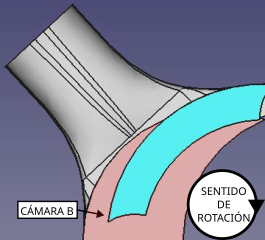
\includegraphics[width=\textwidth]{flujometrias/sin_solape.png}
        \caption{Sin solape}
    \end{subfigure}%
    \begin{subfigure}[t]{0.4\textwidth}
        \centering
        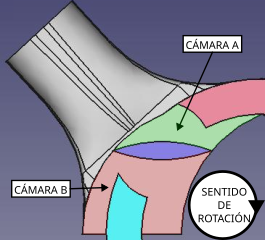
\includegraphics[width=\textwidth]{flujometrias/con_solape.png}
        \caption{Con solape}
    \end{subfigure}
  \caption{Solape de cámaras}\label{fig:solape}
\end{figure}

Independientemente del tipo de flujo que se esté simulando, de ICESym se toman
los valores de presión, temperatura, densidad y velocidad para calcular los
valores iniciales.

Debido a la cantidad de flujometrías a realizar, se utilizó un \emph{script}
para leer los datos de salida de ICESym y calcular los valores requeridos en
función del tipo de flujo a simular.
%
Este \emph{script} toma el estado del gas del simulador tanto en la cámara como
del puerto que se esté analizando, para la posición de alzada y RPM requeridas.
%
De la simulación con ICESym se leen los valores listados en la
Tabla~\ref{tab:valores_iniciales} a partir de los cuales se pueden calcular las
propiedades termodinámicas de la mezcla de gases frescos o quemados,
dependiendo si se está evaluando un puerto de admisión o escape.

Para simplificar el análisis no se tuvo en cuenta la fracción de gases
residuales, el gas ``flujado'' es siempre aire limpio en el caso de los puertos
de admisión o el gas quemado de una mezcla estequiométrica de aire-combustible
en caso de los puertos de escape, siendo isooctano $C_{8}H_{18}$ el combustible
seleccionado.
%
Las ecuaciones utilizadas para modelar las propiedades termodinámicas de las
mezclas aire-combustible fueron descritas brevemente en la
sección~\ref{subsec:prop_mezcla}.
%
Los valores calculados son los indicados en la
Tabla~\ref{tab:valores_calculados}.

\begin{table}
  \centering
  \begin{tabular}{cl}\toprule
    Símbolo & Descripción \\ \midrule
    $\rho_{c,i}$ & es la densidad del gas en la cámara $i$ \\
    $P_{c,i}$ & es la presión del gas en la cámara $i$ \\
    $T_{c,i}$ & es la temperatura del gas en la cámara $i$ \\
    $\rho_{p,i}$ & es la densidad del puerto $i$ \\
    $v_{p,i}$ & es la velocidad del gas en el puerto $i$ \\
    $P_{p,i}$ & es la presión del gas en el puerto $i$ \\ \bottomrule
  \end{tabular}
\caption{Valores iniciales}\label{tab:valores_iniciales}
\end{table}

\begin{table}[h]
  \centering
  \begin{tabular}{cll}\toprule
    Símbolo & Descripción & Ecuación\\ \midrule
    $M_{M}$ & masa molar & \ref{eq:mw} \\
    $C_{p}$ & calor específico a presión constante & - \\
    $\gamma$ & relación $C_{p}/C_{v}$ del gas & - \\
    $\mu$ & viscosidad dinámica & \ref{eq:mu} \\
    $\nu$ & viscosidad cinemática & - \\
    $P_{R}$ & número de Prandtl & \ref{eq:pr} \\
    $k_{est}$ & energía cinética turbulenta & \ref{eq:kappa_est} \\
    $\epsilon_{est}$ & disipación de la energía cinética turbulenta & \ref{eq:epsilon_est} \\ \bottomrule
  \end{tabular}
  \caption{Valores calculados}\label{tab:valores_calculados}
\end{table}

\nomenclature[F]{\(M_{M}\)}{Masa molar}
% \nomenclature[F]{\(C_{p}\)}{Calor específico a presión constante}
\nomenclature[F]{\(\gamma\)}{Cociente de calores específicos}
\nomenclature[F]{\(\mu\)}{Viscosidad dinámica}
\nomenclature[F]{\(\nu\)}{Viscosidad cinemática}
\nomenclature[F]{\(P_{R}\)}{Número de Prandtl}
% \nomenclature[F]{\(k_{est}\)}{Energía cinética turbulenta}


\subsection{Malla}

La malla se construyó a partir del modelo de CAD generado con los resultados
obtenidos de las simulaciones del motor.
%
La implementación de las diferentes herramientas requeridas para generar una
malla apta para realizar las flujometrías se describe en el
apartado~\ref{sec:cap3_of_malla}.

El grado de refinamiento de la malla utilizada para modelar el dominio de la
flujometría tiene un impacto directo en la calidad de los resultados ya que
está relacionado con el error de discretización.
%
Por otro lado, mallas con un alto nivel de refinamiento implican un mayor costo
computacional y dado la cantidad de flujometrías que requiere el trabajo se
optó por determinar un nivel de refinamiento que devuleva una diferencia
relativa entre dos mallas consecutivas no mayor al $5\%$.

Para los puertos de admisión se seleccionó la geometría representada en la
Figura~\ref{fig:refinamiento_admision}.
%
En esta posición hay dos cámaras activas, una con el ciclo en $0^{\circ}$ y
otra a $120^{\circ}$.
%
Las condiciones iniciales se determinan a partir de datos del simulador con el
motor girando a 2000 RPM.%
%
Para los puertos de escape se seleccionó la geometría representada en la
Figura~\ref{fig:refinamiento_escape}.
%
Esta posición corresponde a un período de solape de los puertos con dos cámaras
activas ubicadas en $420^{\circ}$ y $540^{\circ}$.
%
Las condiciones inciales se determinan de los datos de ICESym con el motor
girando a 4000 RPM.

Ambos puertos se simularon con tamaños de malla iniciales de 20, 10, 5 y 2,5 mm,
evaluando la variación del caudal con la cantidad de celdas de la malla, ver
Figura~\ref{fig:refinamiento_admision} para el puerto de admisión y
Figura~\ref{fig:refinamiento_escape} para el puerto de escape.
%
En las Tablas~\ref{tab:convergencia_malla_admision}
y~\ref{tab:convergencia_malla_escape} se presentan los resultados de los
refinamientos junto con el error relativo entre refinamientos sucesivos.

No se observa gran diferencia entre los casos de 20mm a 2,5mm pese a que la
cantidad de celdas es más de 18 veces mayor.
%
Esto se debe a que el software utilizado para realizar el mallado se configuró
para realizar un refinamiento de todas las superficies y bordes, para captar la
geometría de los puertos.
%
En la Figura~\ref{fig:conv_malla_admision} o~\ref{fig:conv_malla_escape} se
puede apreciar la diferencia de tamaño entre las celdas cercanas a las paredes
del puerto y las celdas pertenecientes al interior del volumen para la malla
con tamaño inicial de 20mm.

\begin{table}
  \centering
  \begin{tabular}{cccccc}\toprule
    Tamaño de celda & $N^{\circ}$ Celdas & $Q_{0^{\circ}} [dm^{3}/seg]$ & $\varepsilon_{r,0^{\circ}}$ & $Q_{120^{\circ}} [cm^{3}/seg]$ & $\varepsilon_{r,120^{\circ}}$ \\ \midrule
    20mm  & 20680  & 16,335 & -        & -22,216 & - \\
    10mm  & 53948  & 15,855 & $3,03\%$ & -22,649 & $1,91\%$ \\
    5mm   & 172853 & 15,58  & $1,76\%$ & -23,323 & $2,89\%$ \\
    2,5mm & 389980 & 15,395 & $1,20\%$ & -23,401 & $0,34\%$ \\ \bottomrule
  \end{tabular}
  \caption{Figura~\ref{fig:conv_malla_admision} tabulada}\label{tab:convergencia_malla_admision}
\end{table}

\begin{table}
  \centering
  \begin{tabular}{cccccc}\toprule
    Tamaño de celda & $N^{\circ}$ Celdas & $\dot{m}_{420^{\circ}} [g/seg]$ & $\varepsilon_{r,420^{\circ}}$ & $\dot{m}_{540^{\circ}} [g/seg]$ & $\varepsilon_{r,540^{\circ}}$ \\ \midrule
    20mm  & 31933  & -78,325 & - & -70,43 & - \\
    10mm  & 83817  & -82,048 & 4,54\% & -75,075 & 6,19\% \\
    5mm   & 234487 & -84,44  & 2,83\% & -78,626 & 4,52\% \\
    2,5mm & 676850 & -83,897 & 0,65\% & -76,766 & 2,42\% \\ \bottomrule
  \end{tabular}
  \caption{Figura~\ref{fig:conv_malla_escape} tabulada}\label{tab:convergencia_malla_escape}
\end{table}

\begin{figure}
  \centering
  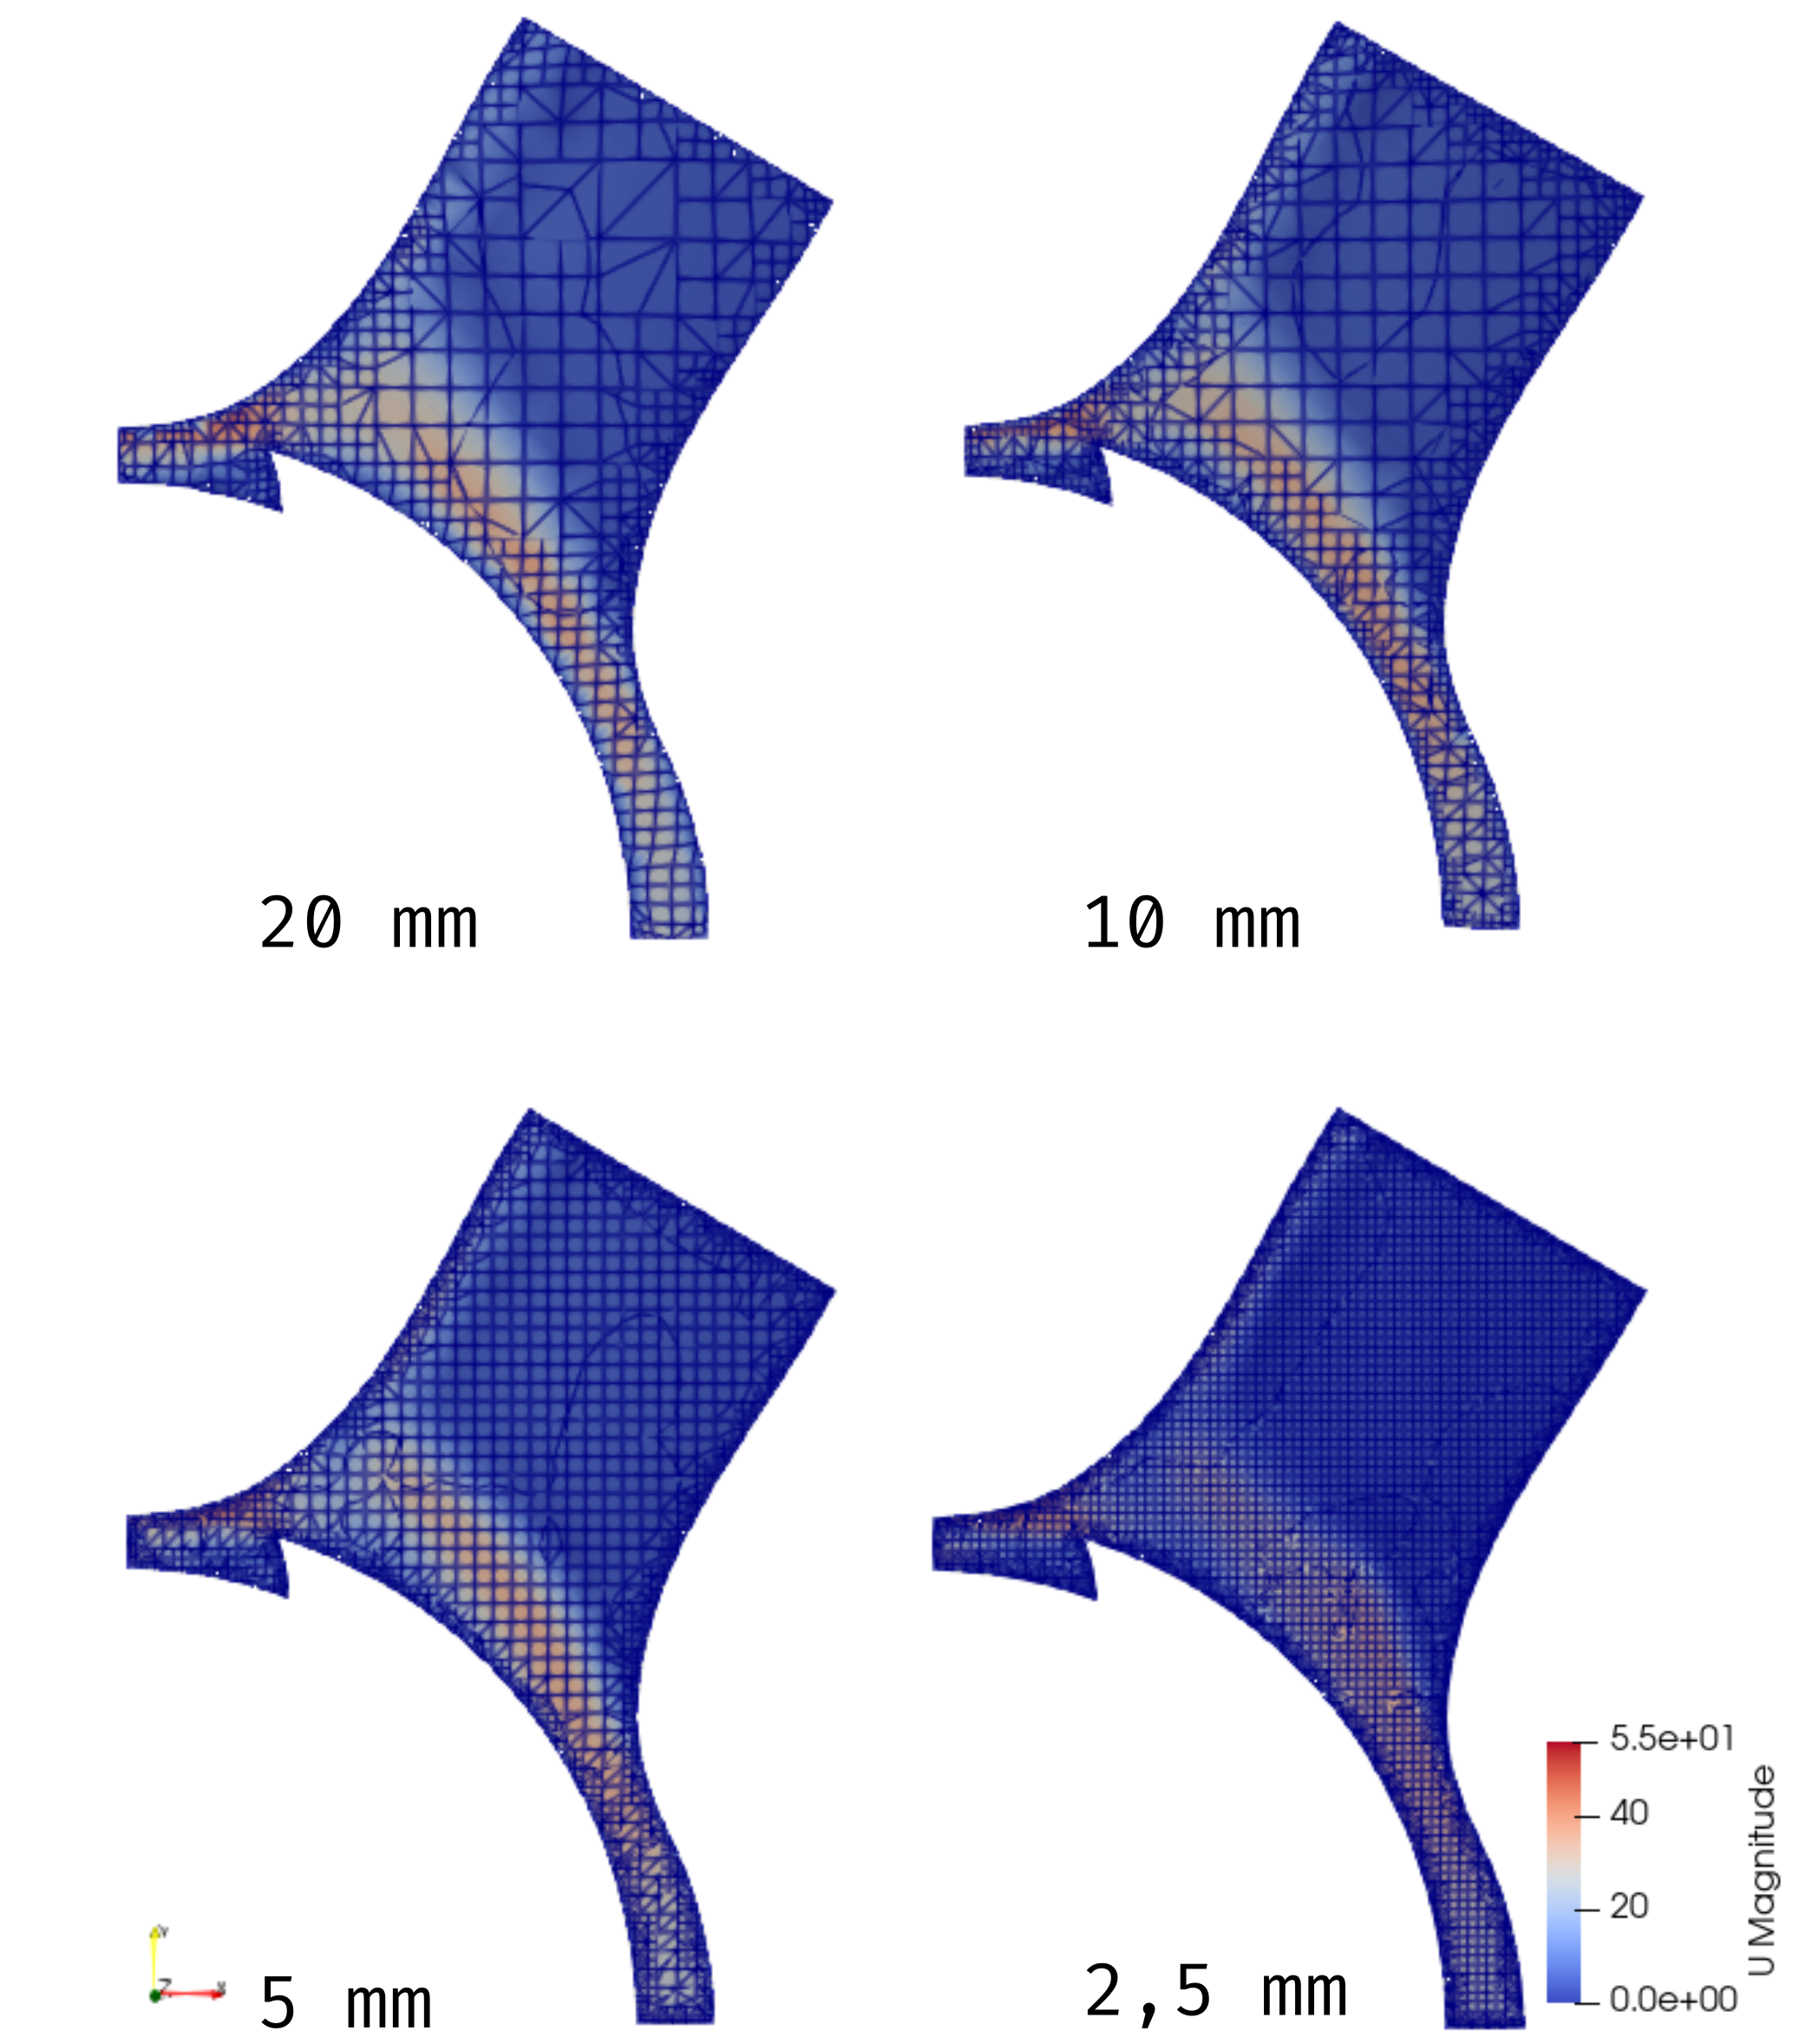
\includegraphics[width=0.8\textwidth]{./flujometrias/refinamiento_malla_admision.png}
  \caption{Refinamiento de malla para puerto de admisión}\label{fig:refinamiento_admision}
\end{figure}

\begin{figure}
  \centering
  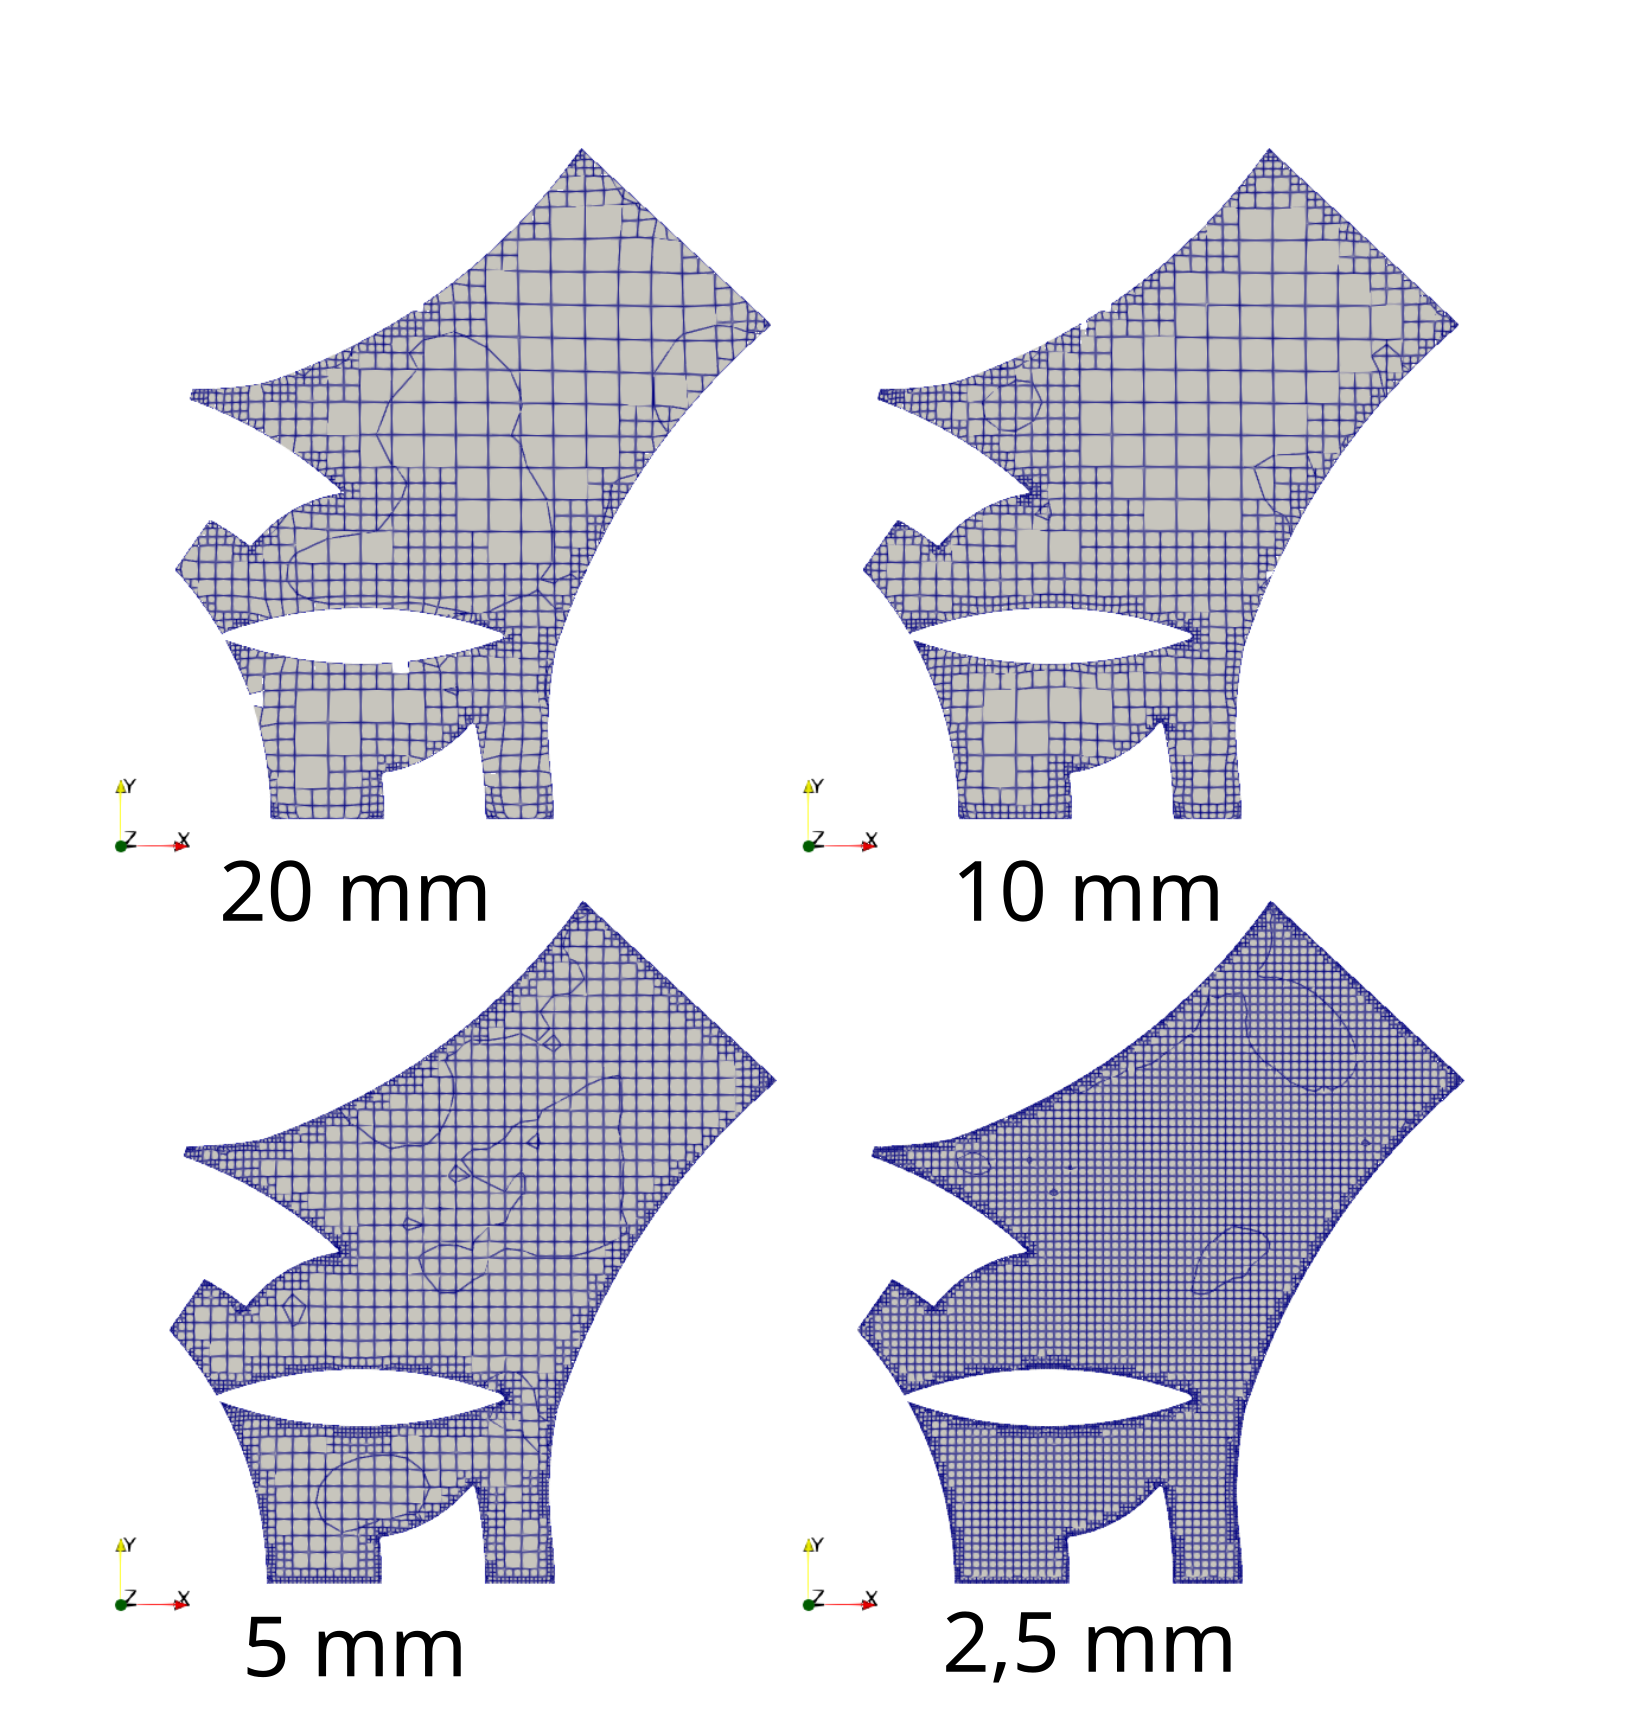
\includegraphics[width=0.8\textwidth]{./flujometrias/refinamiento_malla_escape.png}
  \caption{Refinamiento de malla para puerto de escape}\label{fig:refinamiento_escape}
\end{figure}

\begin{figure}
  \centering
  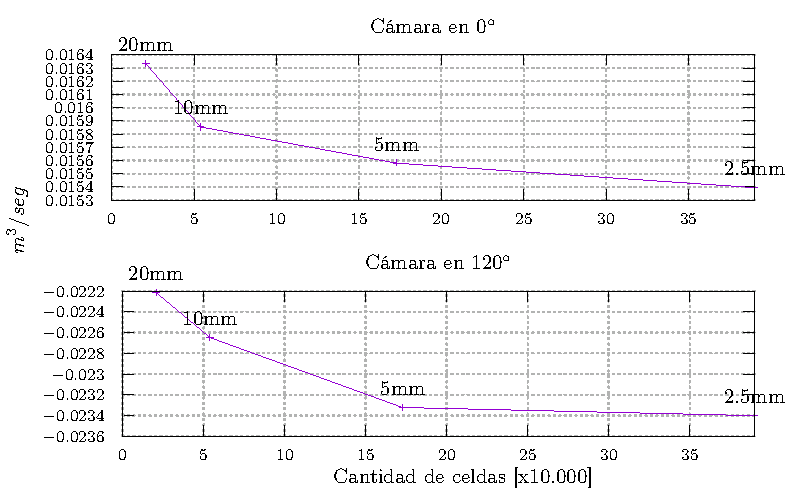
\includegraphics[width=0.9\textwidth]{./flujometrias/convergencia_admision_2000rpm.pdf}
  \caption{Convergencia de malla de puerto de admisión}\label{fig:conv_malla_admision}
\end{figure}

\begin{figure}
  \centering
  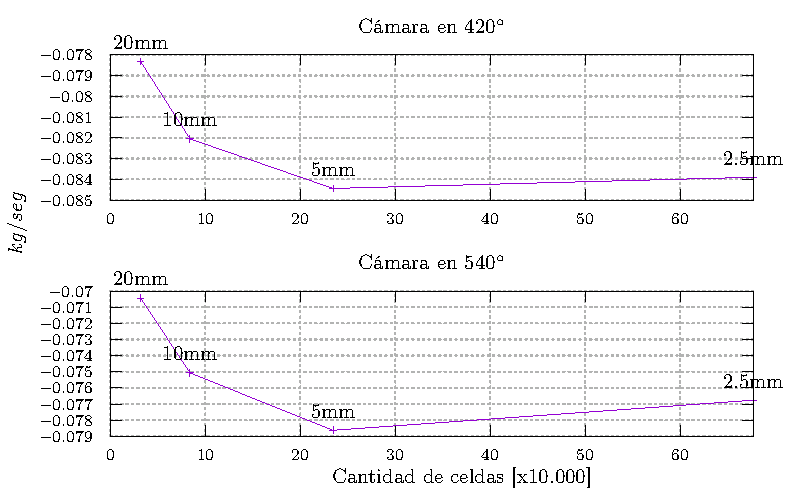
\includegraphics[width=0.9\textwidth]{./flujometrias/convergencia_escape_4000rpm.pdf}
  \caption{Convergencia de malla de puerto de escape}\label{fig:conv_malla_escape}
\end{figure}



\subsection{Esquemas de Discretización Seleccionados}

Los esquemas de discretización utilizados para los casos de \textbf{flujo incompresible} y \textbf{flujo compresible} se resumen en las siguientes tablas.

\begin{table}[h!]
    \centering
    \caption{Esquemas de discretización para flujo incompresible}
    \begin{adjustbox}{max width=\textwidth}
    \begin{tabular}{|l|l|}
        \hline
        \textbf{Componente} & \textbf{Esquema} \\ \hline
        Tiempo & Euler hacia atrás \\ \hline
        Gradiente &
        \begin{tabular}[c]{@{}l@{}}
            $\nabla p$: Integración Gaussiana con interpolación lineal \\
            $\nabla U$: Integración Gaussiana con interpolación lineal
        \end{tabular} \\ \hline
        Divergencia &
        \begin{tabular}[c]{@{}l@{}}
            $\nabla\cdot (\phi U)$: Integración Gaussiana con interpolación lineal \\
            de segundo orden, hacia adelante limitada con $\nabla U$ \\ \hline
            $\nabla\cdot (\phi k)$: Integración Gaussiana con interpolación \\
            lineal hacia adelante \\ \hline
            $\nabla\cdot (\phi \epsilon)$: Integración Gaussiana hacia \\
            adelante con interpolación lineal \\ \hline
            $\nabla\cdot (\phi R)$: Integración Gaussiana con interpolación \\
            lineal \\ \hline
            $\nabla\cdot R$: Integración Gaussiana con interpolación lineal \\ \hline
            $\nabla\cdot \nu_{eff}$: Integración Gaussiana con interpolación lineal
        \end{tabular} \\ \hline
        Laplacianos & Integración Gaussiana con interpolación lineal \\ \hline
        Interpolación & Lineal \\ \hline
        Gradientes normales a la superficie & Sin corregir \\ \hline
    \end{tabular}
    \end{adjustbox}
    \label{tab:esquemas_incompresible}
\end{table}

\begin{table}[h!]
    \centering
    \caption{Esquemas de discretización para flujo compresible}
    \begin{adjustbox}{max width=\textwidth}
    \begin{tabular}{|l|l|}
        \hline
        \textbf{Componente} & \textbf{Esquema} \\ \hline
        Tiempo & Euler \\ \hline
        Gradiente & Integración Gaussiana con interpolación lineal limitada \\ \hline
        Divergencia &
        \begin{tabular}[c]{@{}l@{}}
          $\nabla\cdot (\phi U)$: Integración Gaussiana con interpolación lineal de \\
          segundo orden, hacia adelante limitada con $\nabla U$ \\ \hline
          $\nabla\cdot (\phi, e)$: Integración Gaussiana con interpolación lineal limitada \\ \hline
          $\nabla\cdot (\phi, h)$: Integración Gaussiana con interpolación lineal hacia adelante \\ \hline
          $\nabla\cdot (\phi, p)$: Integración Gaussiana con interpolación lineal limitada \\ \hline
          $\nabla\cdot (\phi, K)$: Integración Gaussiana con interpolación lineal \\ \hline
          $\nabla\cdot (\phi, k)$: Integración Gaussiana con interpolación lineal \\ \hline
          $\nabla\cdot (\phi, \epsilon)$: Integración Gaussiana con interpolación lineal hacia adelante \\ \hline
          $\nabla\cdot (((\rho\cdot \nu_{Eff}) dev2((\nabla U)^{T})))$: Integración Gaussiana \\
          con interpolación lineal \\
        \end{tabular} \\ \hline
        Laplacianos & Integración Gaussiana con interpolación lineal, limitada y corregida \\ \hline
        Interpolación & Lineal \\ \hline
        Gradientes normales a la superficie & Corregida \\ \hline
    \end{tabular}
    \end{adjustbox}
    \label{tab:esquemas_compresible}
\end{table}

En las expresiones anteriores $\phi$ es el flujo volumétrico en la cara de la celda para flujo
incompresible y el flujo másico en la cara de la celda para flujo compresible.
%
\textbf{R} es el tensor de tensiones de Reynolds.

\section{Uso de OpenFOAM}

En esta sección se detalla la configuración, pre-procesado y detalles de la
malla utilizadas en OpenFOAM.

\subsection{Configuración}
%
Para configurar una simulación de OpenFOAM se organiza el directorio de
simulación como se indica en la Figura~\ref{fig:direc_pf} para las flujometrías
de gas considerado como incompresible  y~\ref{fig:direc_rpf} en los casos en
los que se tiene en cuenta la compresibilidad del gas.
%
Cada directorio contiene una carpeta con condiciones iniciales ``0'', malla
``constant'', configuraciones particulares de cada solver ``system'' y una
carpeta con los resultados del post-procesado el cual se puede realizar
durante cada paso de simulación o al final del proceso dependiendo de la
configuración que se haya utilizado.

\begin{figure}[h!]
  \centering
  \begin{subfigure}[b]{0.4\textwidth}
    \centering
    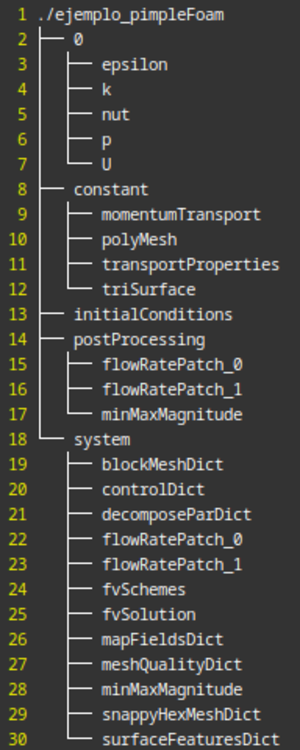
\includegraphics{flujometrias/direct_pimplefoam.pdf}
    \caption{\emph{pimpleFoam}\label{fig:direc_pf} }
  \end{subfigure}%
  \begin{subfigure}[b]{0.4\textwidth}
    \centering
    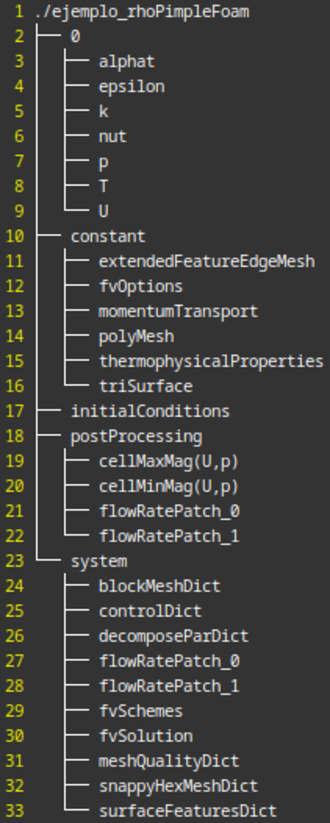
\includegraphics{flujometrias/direct_rhopimplefoam.pdf}
    \caption{\emph{rhoPimpleFoam}\label{fig:direc_rpf} }
  \end{subfigure}
  \caption{Esquema de directorios OpenFOAM}
\end{figure}


En el directorio ``0'' se indican las condiciones iniciales y de borde de cada
simulación, utilizando una configuración genérica con parámetros definidos en un
archivo separado.
%
Esto se realiza de este modo para aprovechar las características paramétricas de
OpenFOAM, permitiendo ejecutar una gran cantidad de simulaciones en serie
variando solamente los parámetros definidos en un archivo externo
``inital\_conditions.cc''.

Estos archivos de condiciones inciales se generan con un \emph{script} que toma
valores de las simulaciones de \emph{ICESym}, como se indicó en la
sección~\ref{cap2:cond_iniciales}, en la que también se detallan las ecuaciones
e hipótesis utilizadas para obtener dichos valores.
%
La ejecución de las simulaciones también se automatiza con scripts de
\emph{bash} con los pasos para ejecutar las corridas con \emph{ICESym}.
%
Con los resultados de las simulaciones se procede a calcular/leer la magnitud
del caudal másico, necesario para el cálculo del coeficiente de descarga.


\subsection{Malla}\label{sec:cap3_of_malla}
%
Una vez obtenido el archivo STL se procede a la generación de la malla dentro de
OpenFOAM con \emph{blockMesh} y \emph{snappyHexMesh}.
%
Primero se crea crea una malla con \emph{blockMesh} que  debe contener la
totalidad del volumen del puerto a simular, como se puede en la
Figura~\ref{fig:paraview_blockMesh_stl}.
%
En este paso se define el tamaño de base de la malla y el nivel general de
refinamiento.
%
A partir de estos hexaedros se produce el refinamiento por \emph{castelación}
que consiste en dividir las celdas en hexaedros más pequeños y luego aplicar el
\emph{snapping} para adaptarse a la superficie del volumen que se está
modelando, ver Figura~\ref{fig:openfoam_shm_pasos}.
%

\begin{figure}
    \centering
    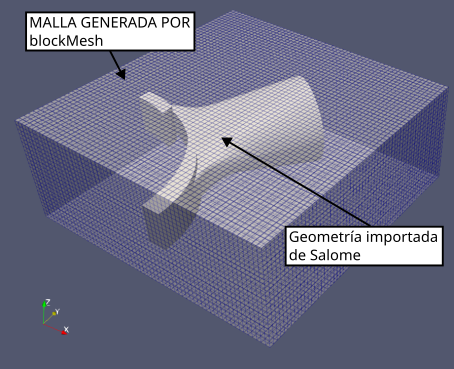
\includegraphics[width=0.5\textwidth]{flujometrias/paraview_blockMesh_stl.png}
    \caption{Malla de blockMesh y stl de Salome}\label{fig:paraview_blockMesh_stl}
\end{figure}

\begin{figure}[t!]
    \centering
    \begin{subfigure}[t]{0.5\textwidth}
        \centering
        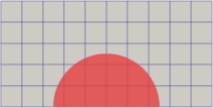
\includegraphics{flujometrias/shm_fondo.png}
        \caption{Malla de fondo y geometría}
    \end{subfigure}%
    \begin{subfigure}[t]{0.5\textwidth}
        \centering
        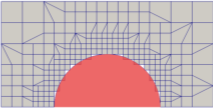
\includegraphics{flujometrias/shm_castelacion.png}
        \caption{Castelación}
    \end{subfigure}
    \begin{subfigure}[t]{0.5\textwidth}
        \centering
        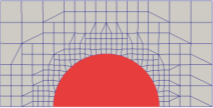
\includegraphics{flujometrias/shm_snapping.png}
        \caption{Snapping}
    \end{subfigure}
    \caption{Pasos de SnappyHexMesh\parencite{shm_steps}}\label{fig:openfoam_shm_pasos}
\end{figure}

El complemento \emph{blockMesh} crea una malla paramétrica con bloques, con
opciones para la creación de la malla con gradientes de tamaño de bloques y
diferentes opciones para los bordes, los cuales se pueden construir por líneas
rectas, arcos o
``splines''.\footnote{\url{https://doc.cfd.direct/openfoam/user-guide-v11/blockmesh}}
%
La malla se genera o configura con un diccionario \emph{blockMeshDict} ubicado
en \emph{constant/polyMesh}, con el cual se construye un cubo capaz de contener
la geometría del puerto a simular.

El complemento \emph{snappyHexMesh}
\footnote{\url{https://doc.cfd.direct/openfoam/user-guide-v11/snappyhexmesh}} es
el segundo paso del mallado.
%
Parte de una malla de bloques como la generada con la utilidad \emph{blockMesh}
y la \emph{talla} para acomodarse a la geometría dada, generando una malla 3D
conformada por hexaedros y hexaedros partidos a partir de superficies de caras
triangulares en formato de \emph{estereolitografía} (STL por sus siglas en
inglés).
%
Además permite refinar zonas particulares de la geometría y crear un
refinamiento mayor en la zona de la capa límite.

Una vez obtenido el archivo STL se procede a la generación de la malla dentro de
OpenFOAM con \emph{blockMesh} y \emph{snappyHexMesh}.
%
Primero se crea crea una malla con \emph{blockMesh} que  debe contener la
totalidad del volumen del puerto a simular, como se puede en la
Figura~\ref{fig:paraview_blockMesh_stl}.
%
En este paso se define el tamaño de base de la malla y el nivel general de
refinamiento.
%
A partir de estos hexaedros se produce el refinamiento por \emph{castelación}
que consiste en dividir las celdas en hexaedros más pequeños y luego aplicar el
\emph{snapping} para adaptarse a la superficie del volumen que se está
modelando, ver Figura~\ref{fig:openfoam_shm_pasos}.
%

\subsection{Pre-procesado}
%
El preprocesado consiste en definir geometría y condiciones iniciales de la
simulación a partir de los datos obtenidos de las simulaciones con el
optimizador e ICESym.
%
Con los resultados del simulador se grafica la diferencia de presión entre el
puerto de admisión o escape y la cámara correspondiente en función de la apertura
del puerto, para un rango de velocidades de 1000 a 9000 RPM, con el fin de
identificar las zonas en las condiciones operativas en las que evaluar el puerto.
%
En la Figura~\ref{fig:puntos_interes} se muestra una gráfica de $\Delta P$ y
alzada para los puertos de admisión y escape de 1000 a 4000 RPM de un motor
resultante de una de las simulaciones.

Como es de esperarse se tienen mayores diferenciales de presión a menores
aperturas del puerto porque se está próximo a los eventos de apertura o cierre
del mismo.
%
A diferencia del puerto de admisión, en el puerto de escape se ve una banda
bastante definida de operación que se hace más ``llena'' a medida que aumenta la
apertura del puerto.
%
Durante la apertura del puerto se ven las mayores diferencias de presión en las
que hay dos bandas bien definidas.
%
Se toman algunos puntos arriba en la zona con mayor $\Delta P$ y una cantidad
menor para velocidades con $\Delta P \simeq 0$.
%
A medida que el puerto se abre la diferencia de presión con el gas en la cámara
disminuye y esta banda se afina.

\begin{figure}
    \centering
    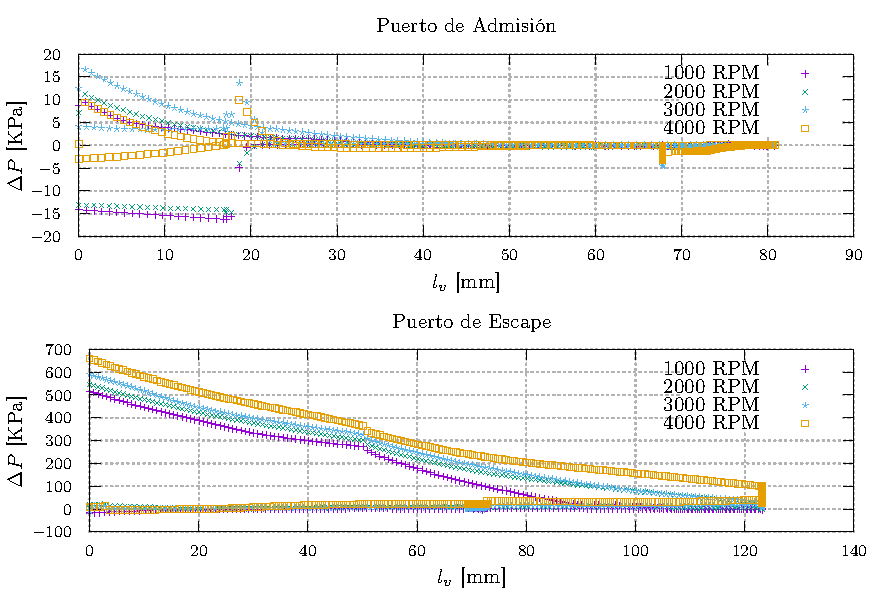
\includegraphics[width=\textwidth]{gnuplot/puntos_interes.pdf}
    \caption{Presión en función de la apertura el puerto,
$\Delta P = f(l_{v})$}\label{fig:puntos_interes}
\end{figure}

El valor de alzada está directamente relacionado con la posición angular del
cigüeñal, por lo que una vez seleccionados los puntos de interés se puede
extraer la geometría deseada de un modelo de CAD paramétrico del motor.
%
En este modelo se representó la mitad de la geometría que contiene los puertos
de admisión y escape, y se obtuvo realizando operaciones geométricas con los
volúmenes que representan diferentes componentes del motor como son el estator,
rotor, paletas, etc.


\begin{figure}
    \centering
    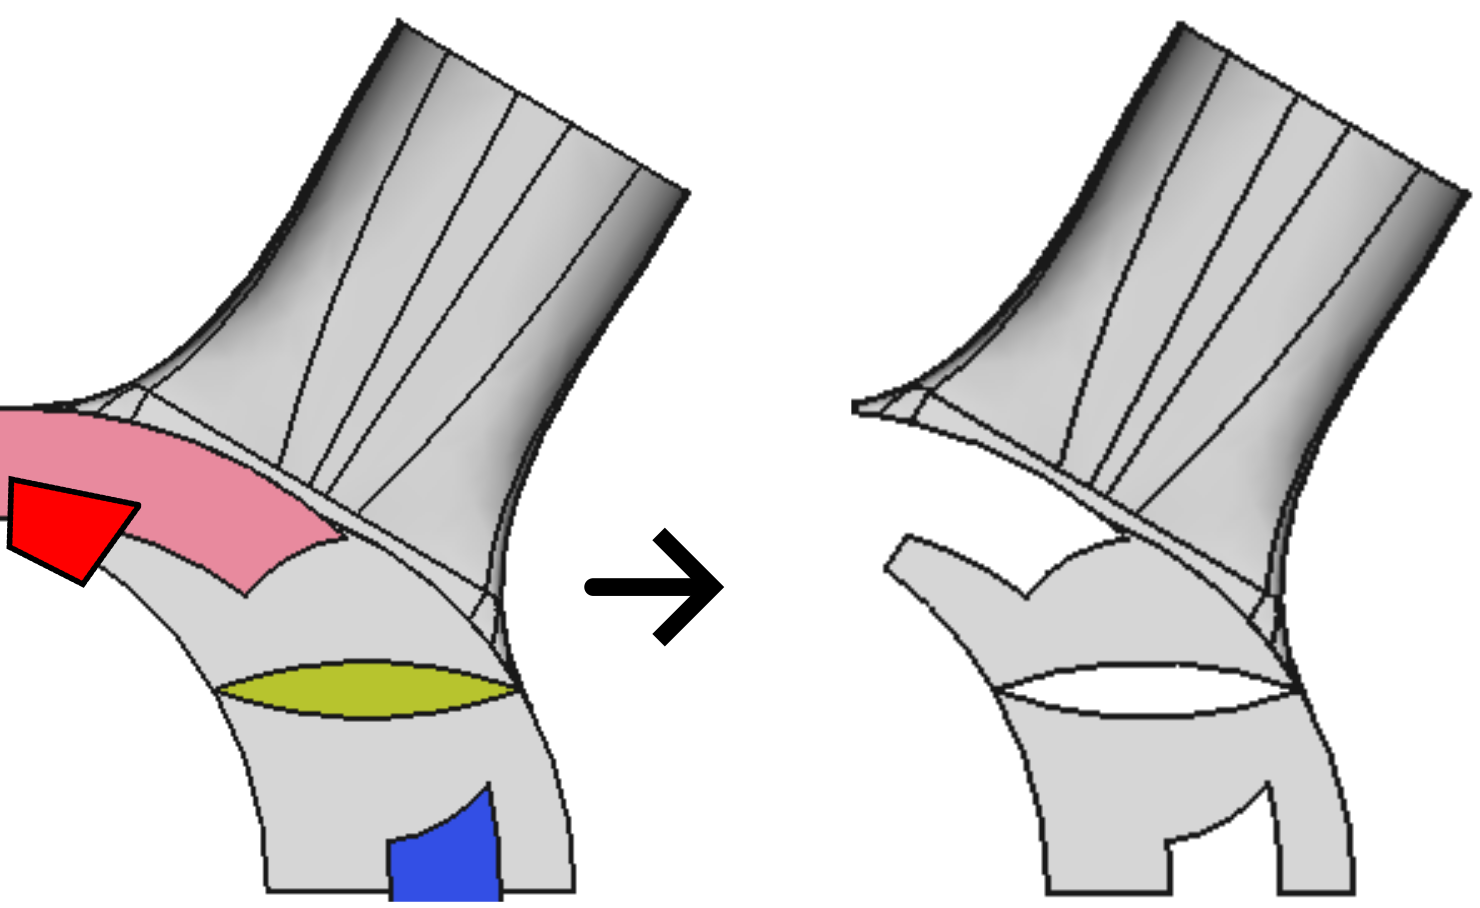
\includegraphics[width=0.7\textwidth]{./CAD/freecad_pasos.png}
    \caption{Puerto de admisión para $\theta=50^{\circ}$ modelado con
FreeCAD}\label{fig:admision_50}
\end{figure}

Esta geometría fue generada por el programa FreeCAD~\parencite{freecad},
exportada a un archivo
``.BREP''\footnote{\href{https://dev.opencascade.org/doc/overview/html/specification\_\_brep\_format.html}{Formato
BREP, opencascade.org}} para luego ser importada en Salome\parencite{salome},
que se utiliza para generar una malla cerrada, hermética, que puede ser
procesada por los complementos de OpenFOAM utilizados para generar la malla de
la simulación.
%
Es importante que se satisfaga la hermeticidad de la malla, lo cual significa
que los nodos en la frontera entre superficies coincidan, como se puede observar
en la Figura~\ref{fig:salome_malla_hermetica}, en la que se ven dos superficies
``walls'' y ``outlet'' y los nodos compartidos entre ambas superficies.
%

\begin{figure}[ht]
    \centering
    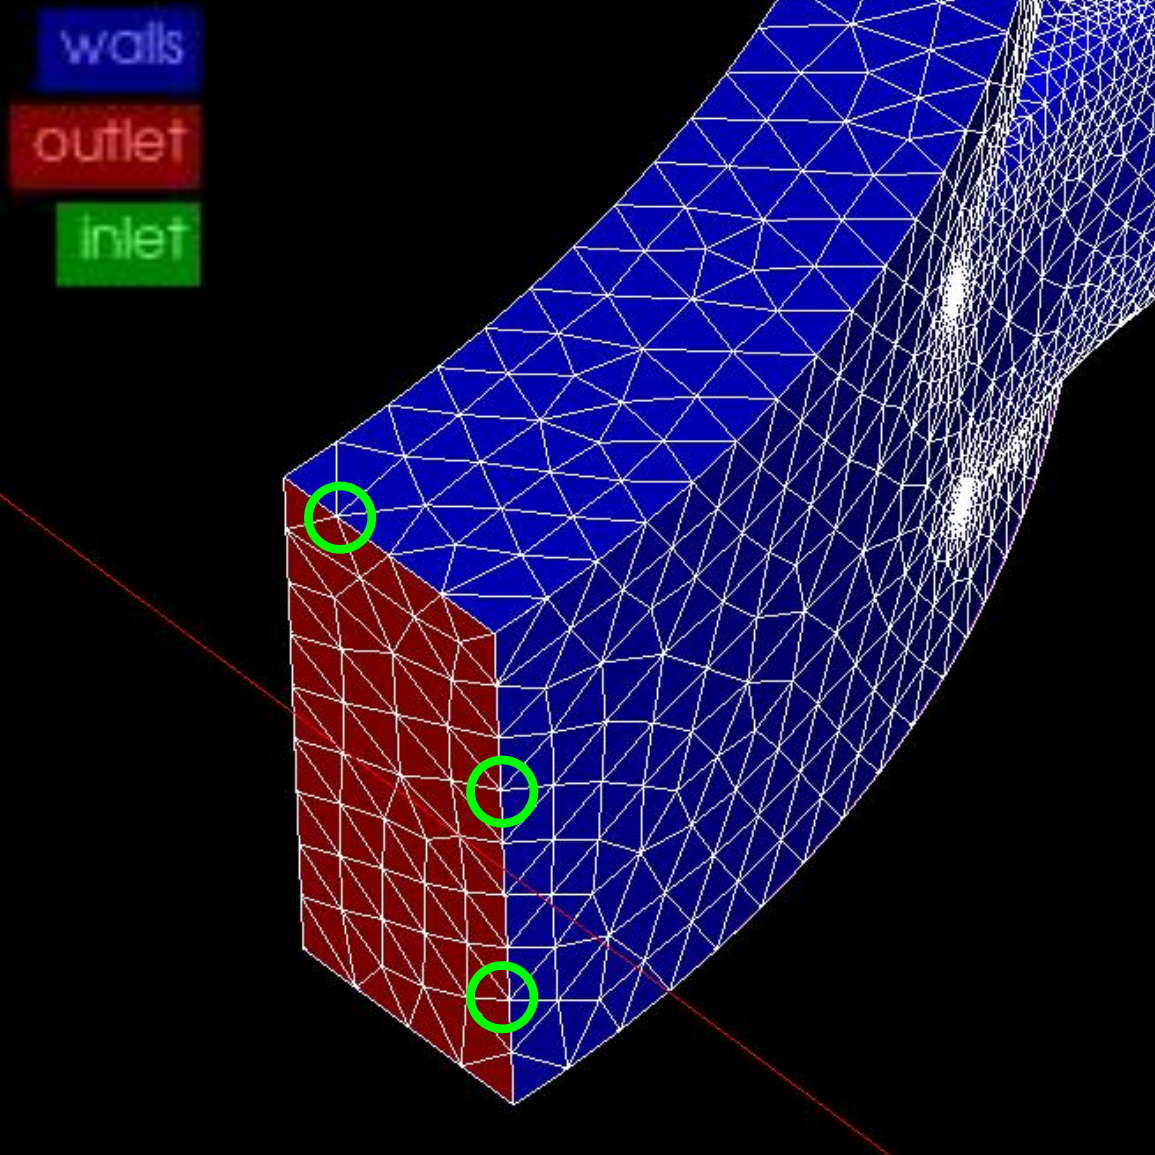
\includegraphics[width=0.4\textwidth]{./flujometrias/salome_malla_hermetica.png}
    \caption{Malla hermética}\label{fig:salome_malla_hermetica}
\end{figure}

El proceso en Salome consta de importar la geometría generada por FreeCAD y
separar la misma en superficies utilizadas para definir condiciones de contorno
en OpenFOAM.
%
Las superficies diferenciadas son: puerto, cámara/s y pared, ver
Figura~\ref{fig:openfoam_parches}.

\begin{figure}[ht]
    \centering
    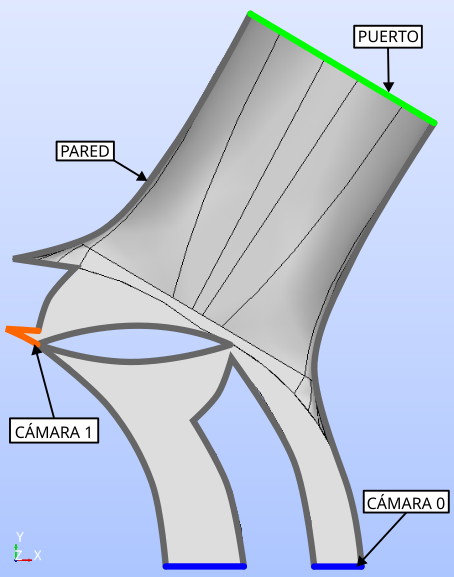
\includegraphics[width=0.5\textwidth]{./flujometrias/openfoam_parches.png}
    \caption{Nombres de Parches}\label{fig:openfoam_parches}
\end{figure}

Luego de separadas estas superficies se procede a generar la malla en formato
ASCII STL con el complemento de mallado de Salome.
%
Se utilizó el generador de mallas NETGEN 1D-2D para crear la superficie, en
general se configuró el software de modo de tener un stl de buena calidad con
elementos de menor tamaño en zonas de mayor curvatura.
%
En la Figura~\ref{fig:salome_fina_gruesa} se ve la diferencia en cantidad de
nodos de dos mallas, una malla fina a la izquierda y una malla gruesa a la
derecha.
%
En la Tabla~\ref{tab:salome_fina_gruesa} se muestra la diferencia entre algunos
parámetros básicos de configuración para las dos mallas.
%
% Esto sin requerir de una gran cantidad de elementos para no ralentizar el
% procesado con SnappyHexMesh.

\begin{figure}[t!]
    \centering
    \begin{subfigure}[t]{0.5\textwidth}
        \centering
        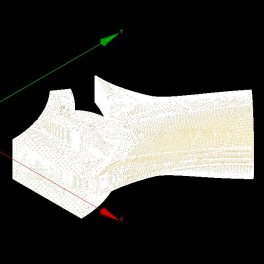
\includegraphics{/flujometrias/salome3_fina.png}
        \caption{Malla fina sin optimizar}
    \end{subfigure}%
    \begin{subfigure}[t]{0.5\textwidth}
        \centering
        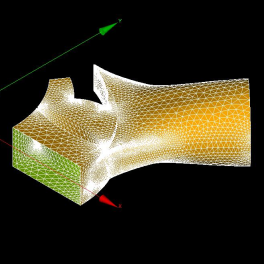
\includegraphics{/flujometrias/salome3_gruesa.png}
        \caption{Malla gruesa optimizada}
    \end{subfigure}
    \caption{Diferentes mallas para flujometrías}\label{fig:salome_fina_gruesa}
\end{figure}

\begin{table}
    \centering
    \begin{tabular}{lccc} \toprule
        Parámetro                & Malla Fina    & Malla Gruesa     & Unidades\\ \midrule
        Tamaño máximo            & 0,001         & 0,03             & m \\
        Tamaño mínimo            & 1E-7          & 2,4E-5           & m \\
        Limitado por curvatura   & Sí            & Sí               & - \\
        Optimizar                & No            & Sí               & - \\
        Cantidad de nodos        & 99311         & 49112            & - \\
        Cantidad de elementos    & 204695        & 103163           & - \\ \bottomrule
    \end{tabular}
    \caption{Configuración de mallas mostradas en la Figura~\ref{fig:salome_fina_gruesa}}
    \label{tab:salome_fina_gruesa}
\end{table}
